\documentclass[8pt]{beamer}


\mode<presentation>
{
\usetheme{Singapore} %use default if problems or Szeged
  % or ... https://deic-web.uab.cat/~iblanes/beamer_gallery/index_by_theme.html
}
\setbeamertemplate{footline}[frame number]
\usepackage{booktabs}
\usepackage{color}

\usepackage[english]{babel}
% or whatever

\usepackage[latin1]{inputenc}
% or whatever

\usepackage{times}
\usepackage[T1]{fontenc}
% Or whatever. Note that the encoding and the font should match. If T1
% does not look nice, try deleting the line with the fontenc.
\usepackage[super]{nth}
\usepackage{xcolor}
\usepackage{relsize} %large math 

\usepackage{graphicx} % to insert the logo

\usepackage[font=scriptsize,skip=1pt]{caption}

\setbeamertemplate{caption}[numbered]

\title[S.I.s.a.R. Model] % (optional, use only with long paper titles)
{An Agent-Based Model to simulate the Covid-19 epidemic diffusion, with the use of Genetic Algorithms to optimize vaccinations}

\author[] % (optional, use only with lots of authors)
{G.~Pescarmona\inst{1} \and P.~Terna\inst{2} \and A.~Acquadro\inst{1} \and P.~Pescarmona\inst{3} \and G.~Russo\inst{4}  
\and S.~Terna\inst{5}  }
% - Give the names in the same order as the appear in the paper.
% - Use the \inst{?} command only if the authors have different
%   affiliation.


\institute[] % (optional, but mostly needed)
{
  \inst{1}%
 University of Torino, Italy
  \and
  \inst{2}%
  University of Torino, Italy, retired \& Fondazione Collegio Carlo Alberto, Honorary Fellow, Italy
 \and
  \inst{3}%
  University of Groningen, The Netherlands  
  \and
  \inst{4}%
  Centro Einaudi, Torino, Italy
  \and
  \inst{5}%
 tomorrowdata.io
  }
% - Use the \inst command only if there are several affiliations.
% - Keep it simple, no one is interested in your street address.


\date[] % (optional, should be abbreviation of conference name)
{CCA -- March \nth{29}, 2021}

\begin{document}

%%%%%%%%%%%%%%%%%%%%%%%%%%%%%%%%%%%%%%%%%%%%%%%%%%%%%%%%%
\begin{frame}


\includegraphics[width=0.18\textwidth]{logo_unito.png}~~~
\includegraphics[width=0.15\textwidth]{CCA_Logo.png}

  \titlepage
\end{frame}

%%%%%%%%%%%%%%%%%%%%%%%%%%%%%%%%%%%%%%%%%%%%%%%%%%%%%%%%%
\begin{frame}{Outline}
  \tableofcontents
  % You might wish to add the option [pausesections]
\end{frame}

%%%%%%%%%%%%%%%%%%%%%%%%%%%%%%%%%%%%%%%%%%%%%%%%%%%%%%%%%
\section{Introduction}

%%%%%%%%%%%%%%%%%%%%%%%%%%%%%%%%%%%%%%%%%%%%%%%%%%%%%%%%%
\begin{frame}{Objectives of the model}

  \begin{itemize}
  \item
We propose an agent-based model to simulate the Covid-19 epidemic diffusion, with Susceptible, Infected, symptomatic, asymptomatic, and Recovered people: hence the name S.I.s.a.R. The scheme comes from S.I.R. models, with (i) infected agents categorized as symptomatic and asymptomatic and (ii) the places of contagion specified in a detailed way, thanks to agent-based modeling capabilities. 

 \item
The infection transmission is related to three factors: the infected person's characteristics and those of the susceptible one, plus those of the space in which contact occurs.

 \item
The model includes the structural data of Piedmont, but it can be readily calibrated for other areas. The model manages a realistic calendar (e.g., national or local government decisions), via a script interpreter.  


 \end{itemize}
\end{frame}

%%%%%%%%%%%%%%%%%%%%%%%%%%%%%%%%%%%%%%%%%%%%%%%%%%%%%%%%%
\begin{frame}{Tool and links}

  \begin{itemize}

\item We use NetLogo, at \url{https://ccl.northwestern.edu/netlogo/}.

 \item
 
S.I.s.a.R. is at \url{https://terna.to.it/simul/SIsaR.html} with information on model construction, the draft of a paper also reporting results, and an online executable version of the simulation program, built using NetLogo.

 \item
 A short paper is published at \url{https://rofasss.org/2020/10/20/sisar/}
 
 G. Pescarmona, P. Terna, A. Acquadro, P. Pescarmona, G. Russo, and S. Terna. How Can ABM Models Become Part of the Policy-Making Process in Times of Emergencies---The SISAR Epidemic Model. \emph{RofASSS}, 2020.

 \end{itemize}
\end{frame}

%%%%%%%%%%%%%%%%%%%%%%%%%%%%%%%%%%%%%%%%%%%%%%%%%%%%%%%%%
\begin{frame}{The scale and the items}

\begin{itemize}

\item $1:1000$.

\bigskip

\item Houses.
\item Schools.
\item Hospitals.
\item Nursing homes,
\item Factories.

\end{itemize}

\end{frame}
%%%%%%%%%%%%%%%%%%%%%%%%%%%%%%%%%%%%%%%%%%%%%%%%%%%%%%%%%
\section{The model}

%%%%%%%%%%%%%%%%%%%%%%%%%%%%%%%%%%%%%%%%%%%%%%%%%%%%%%%%%
\subsection{Overview}

%%%%%%%%%%%%%%%%%%%%%%%%%%%%%%%%%%%%%%%%%%%%%%%%%%%%%%%%%
\begin{frame}{The interface and the information sheet}

\begin{figure}[H]
\center
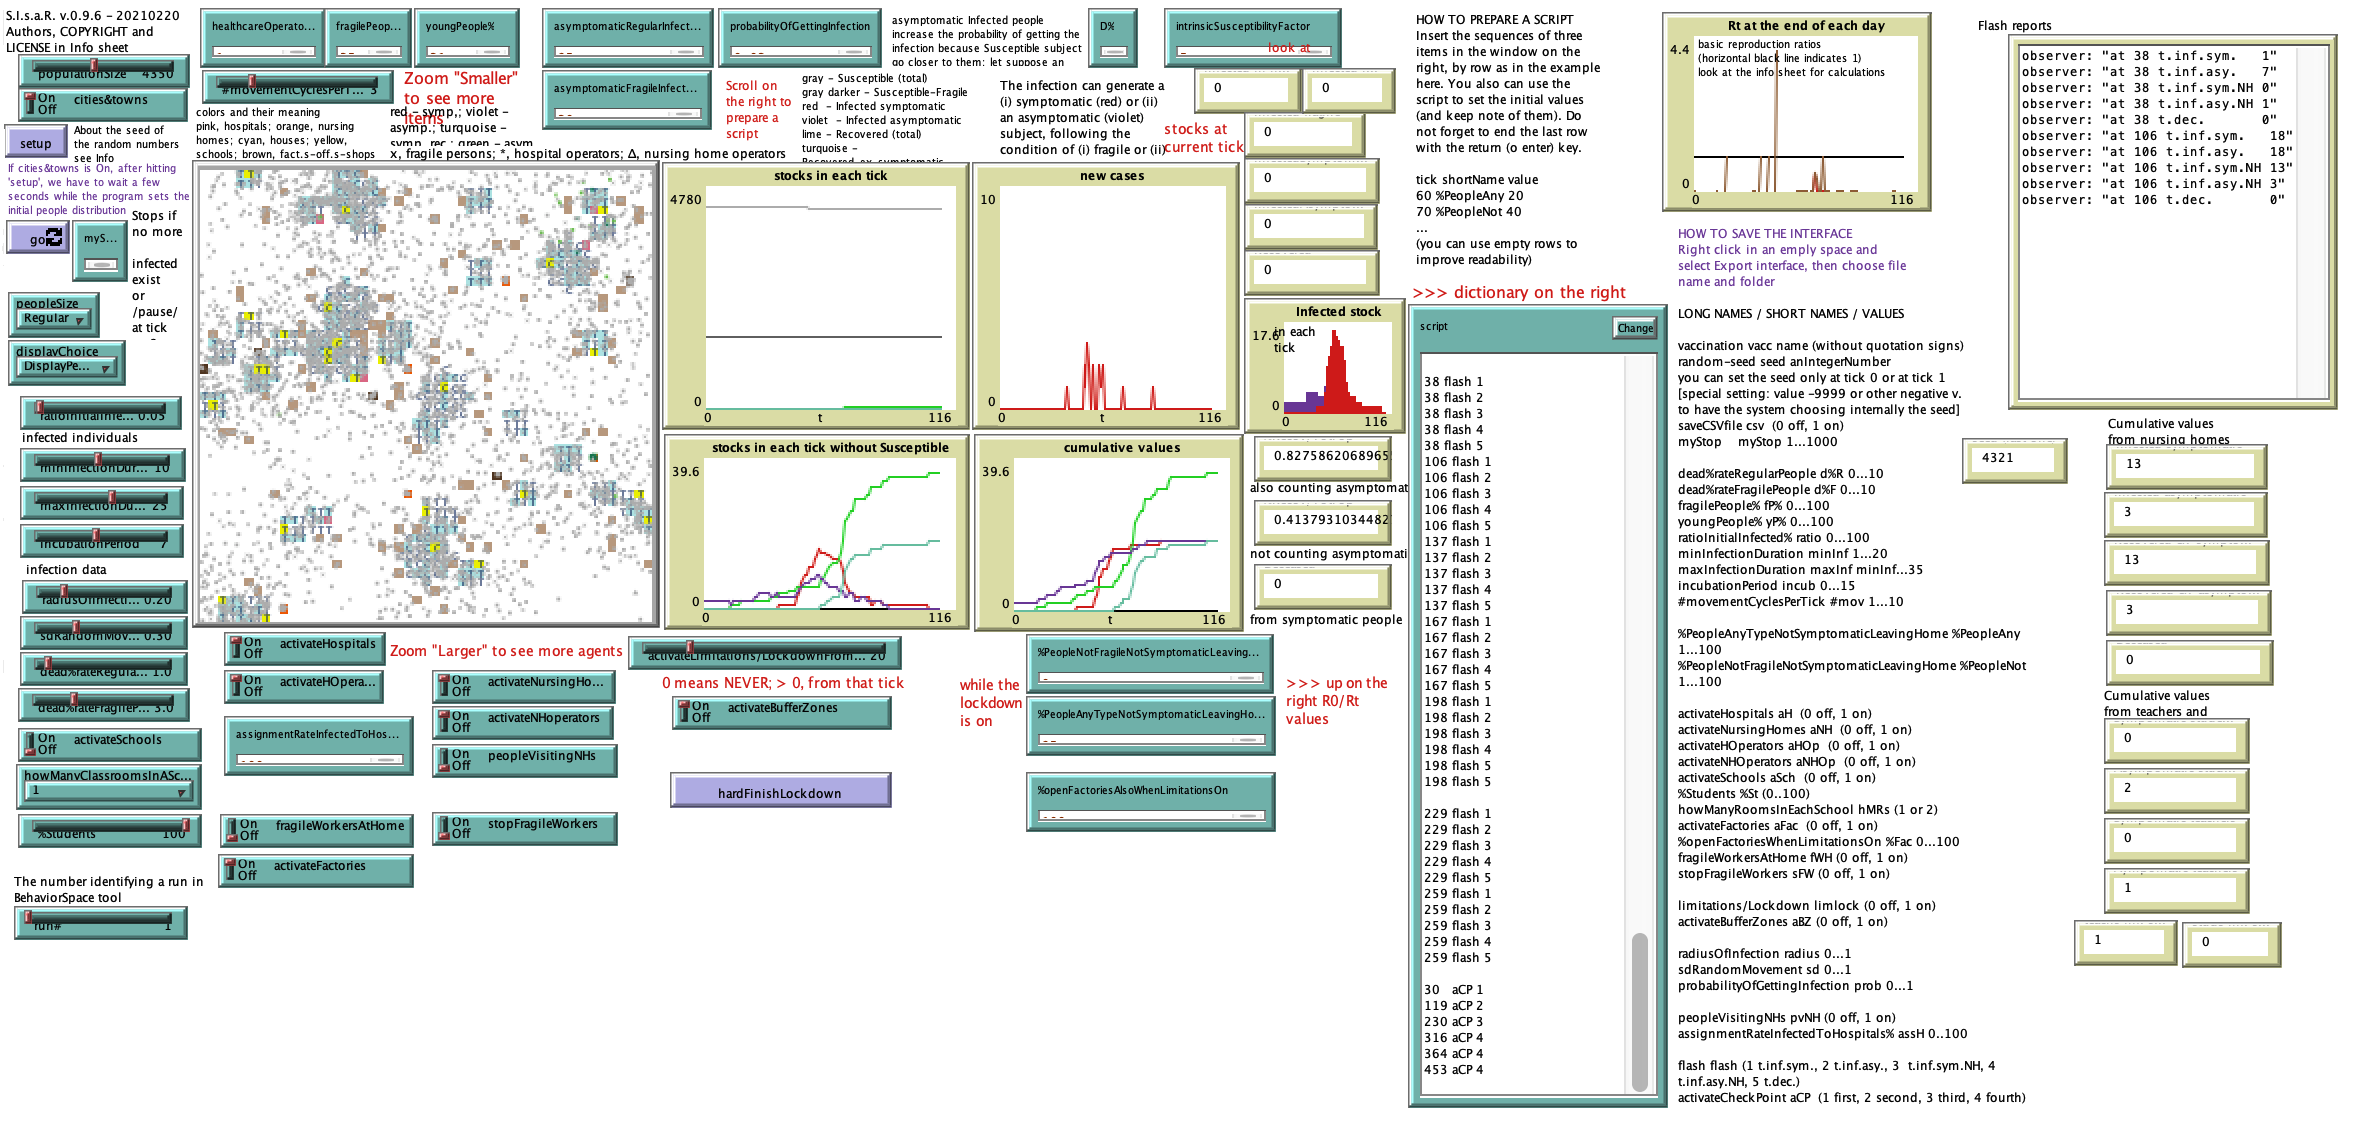
\includegraphics[scale=0.14]{interface2021.png}

\caption{The interface} 
\label{interface}
\end{figure}

\end{frame}

%%%%%%%%%%%%%%%%%%%%%%%%%%%%%%%%%%%%%%%%%%%%%%%%%%%%%%%%%
\begin{frame}{The interface and the information sheet}

\begin{figure}[H]
\center
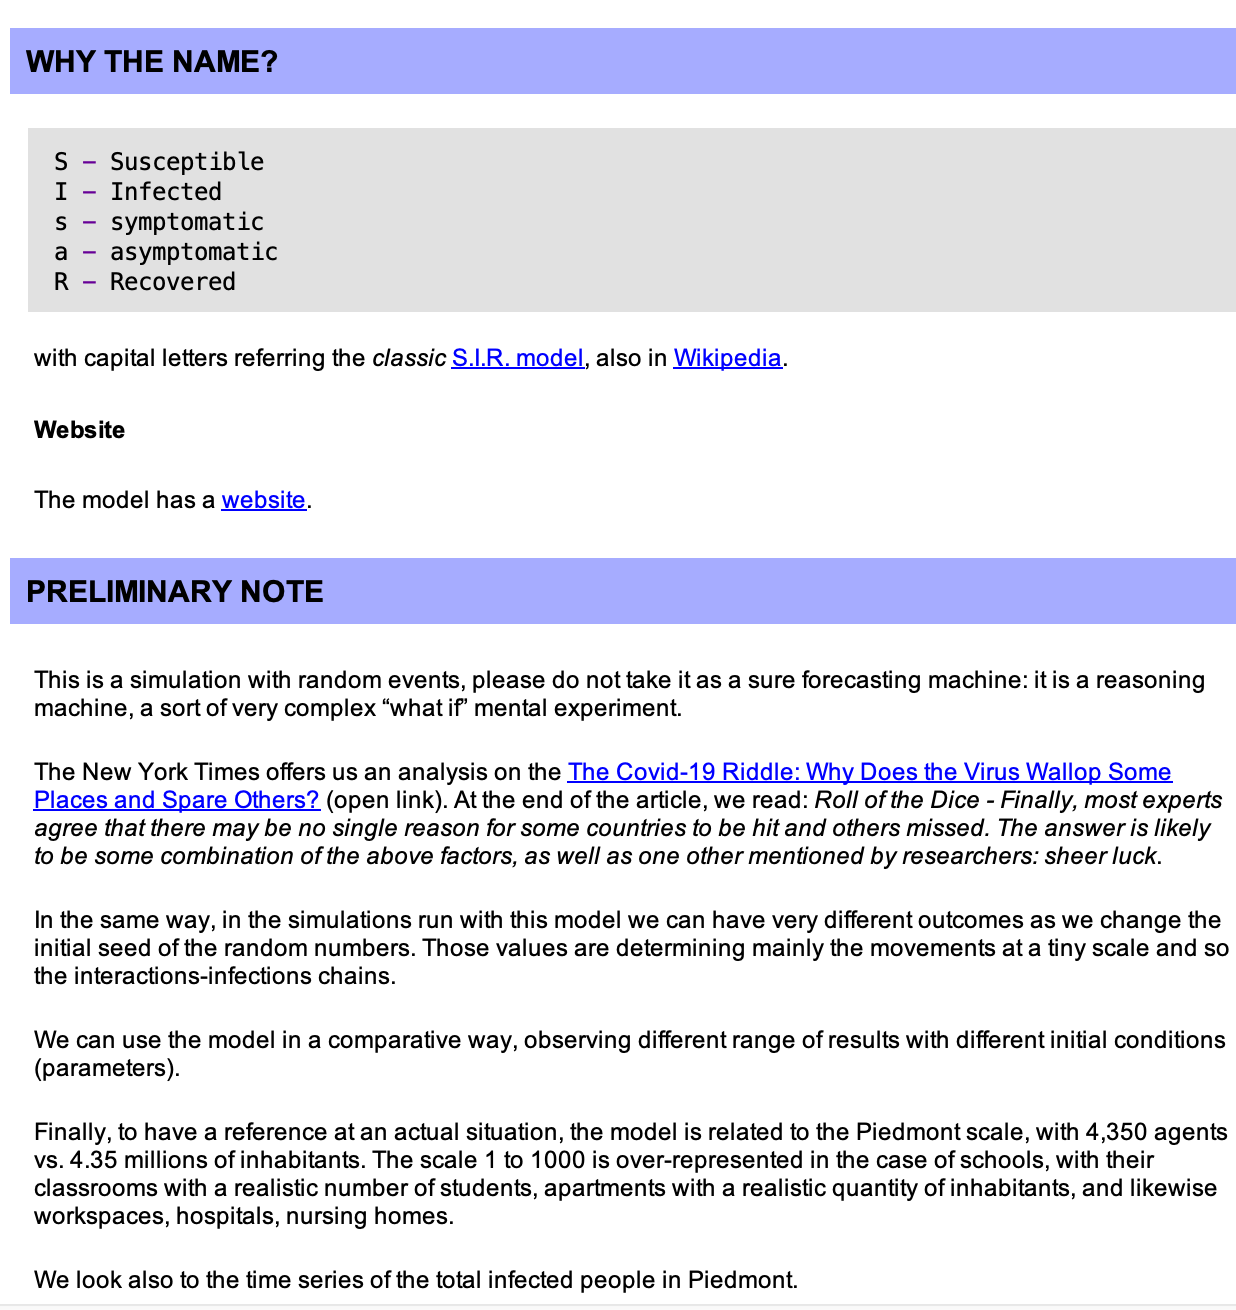
\includegraphics[scale=0.23]{info1b.png}~~~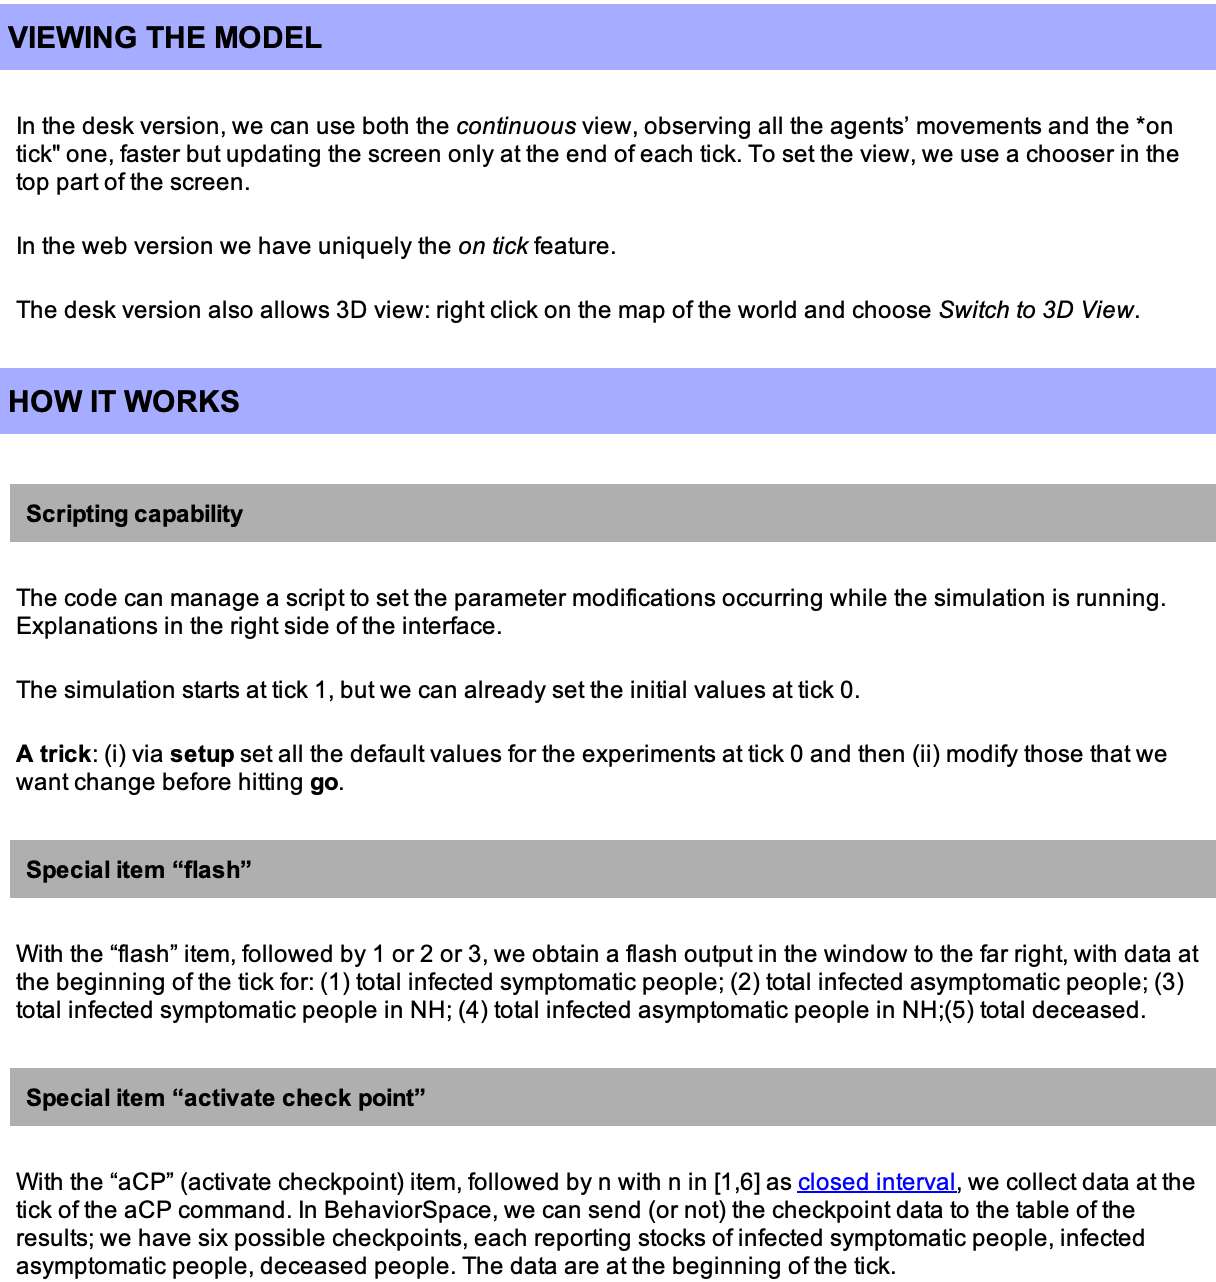
\includegraphics[scale=0.23]{info2b.png}

\caption{The information sheet, about  20 pages} 
\label{interface}
\end{figure}

\end{frame}

%%%%%%%%%%%%%%%%%%%%%%%%%%%%%%%%%%%%%%%%%%%%%%%%%%%%%%%%%
\subsection{Details}

%%%%%%%%%%%%%%%%%%%%%%%%%%%%%%%%%%%%%%%%%%%%%%%%%%%%%%%%%
\begin{frame}{The world}

\begin{figure}[H]
\center
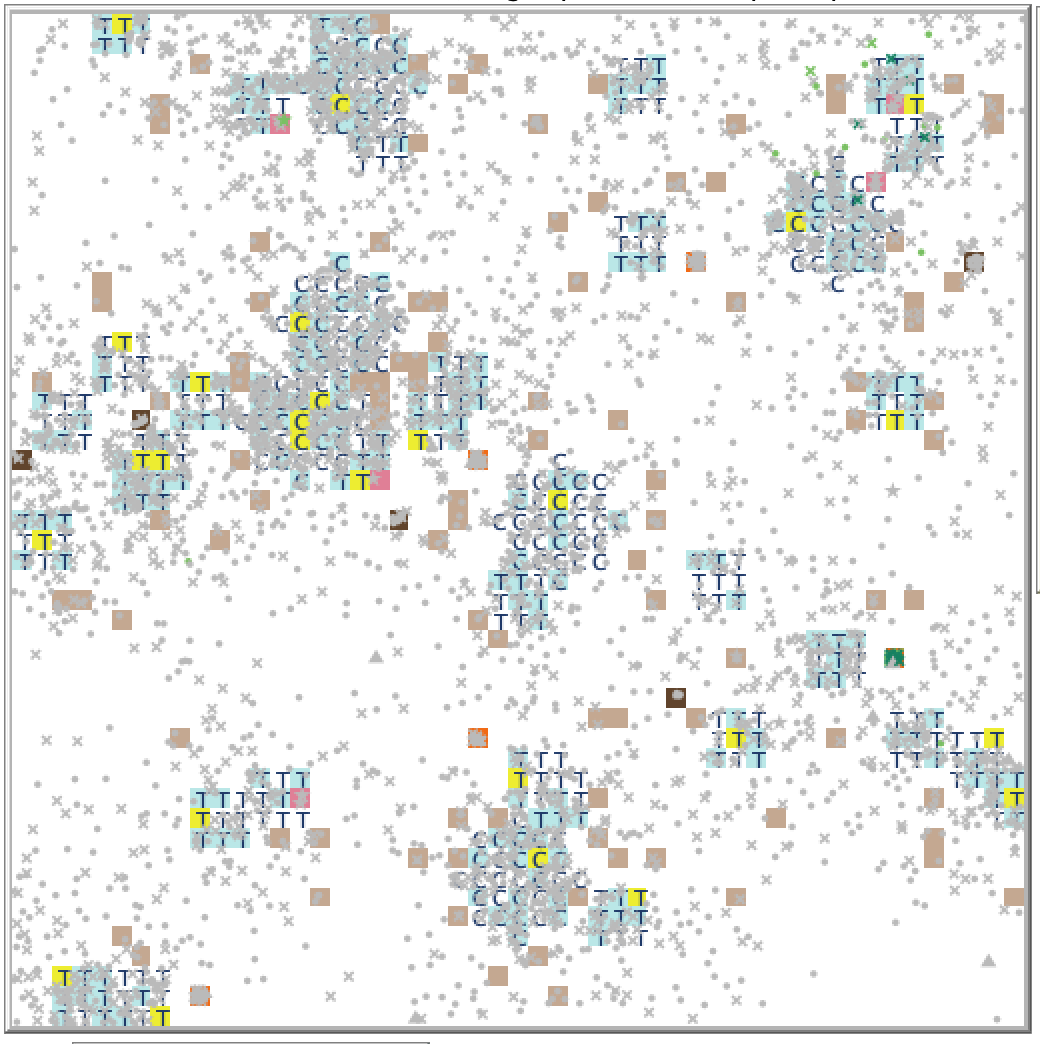
\includegraphics[scale=0.35]{world.png}

\caption{The world} 
\label{world}
\end{figure}

\end{frame}

%%%%%%%%%%%%%%%%%%%%%%%%%%%%%%%%%%%%%%%%%%%%%%%%%%%%%%%%%
\begin{frame}{The world 3D}

\begin{figure}[H]
\center
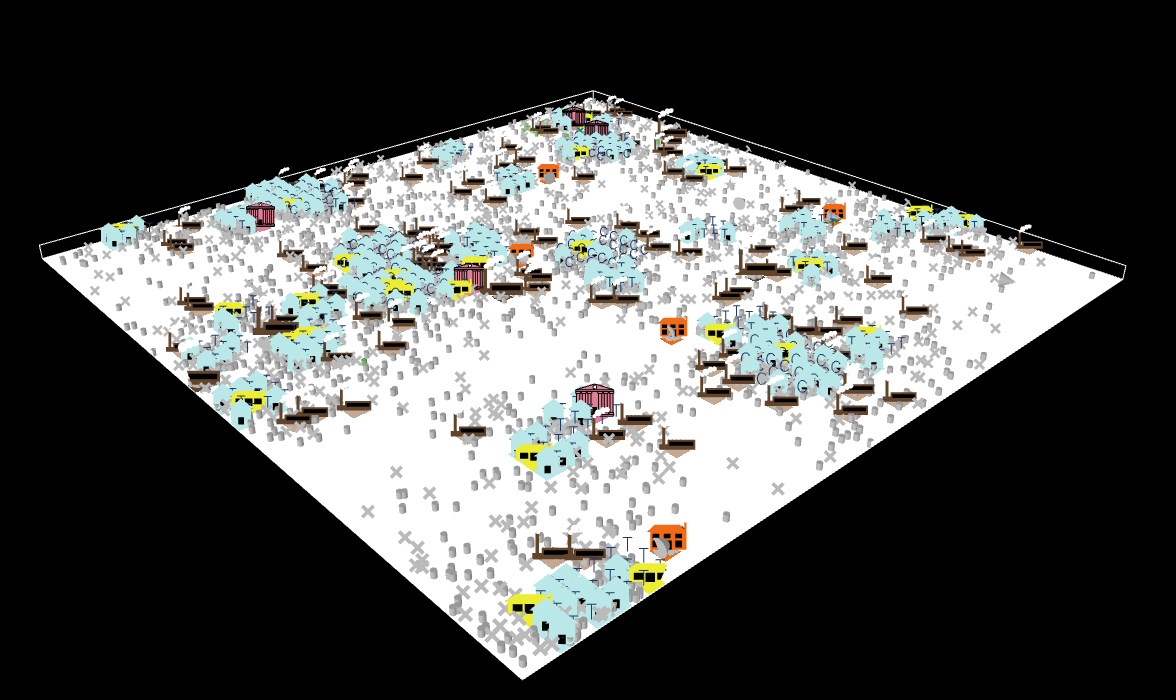
\includegraphics[scale=0.55]{world3D.png}

\caption{The world 3D} 
\label{world3D}
\end{figure}

\end{frame}

%%%%%%%%%%%%%%%%%%%%%%%%%%%%%%%%%%%%%%%%%%%%%%%%%%%%%%%%%
\begin{frame}{The agents}

\begin{figure}[H]
\center
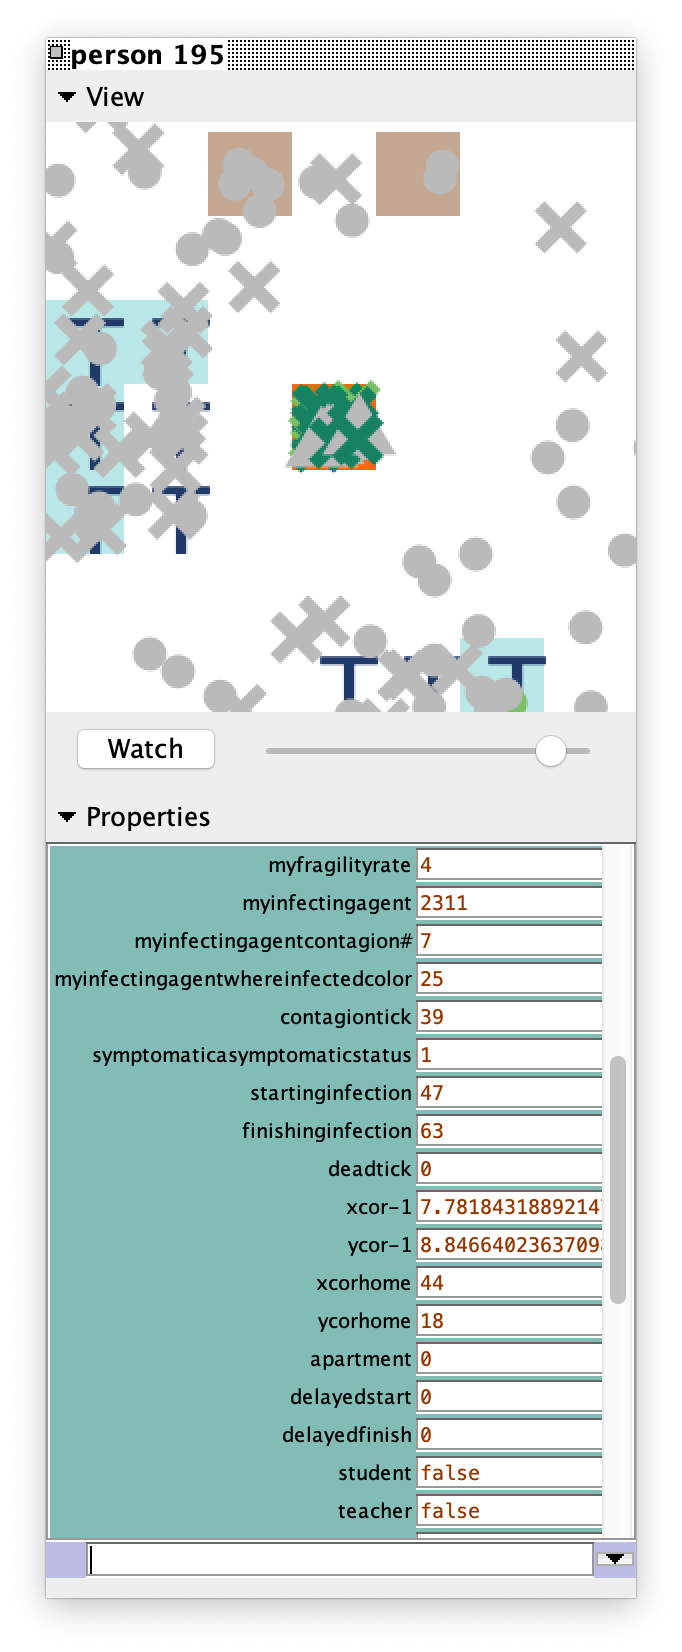
\includegraphics[scale=0.23]{person1.png}~~~~~~~~~~~~~~~~~~~~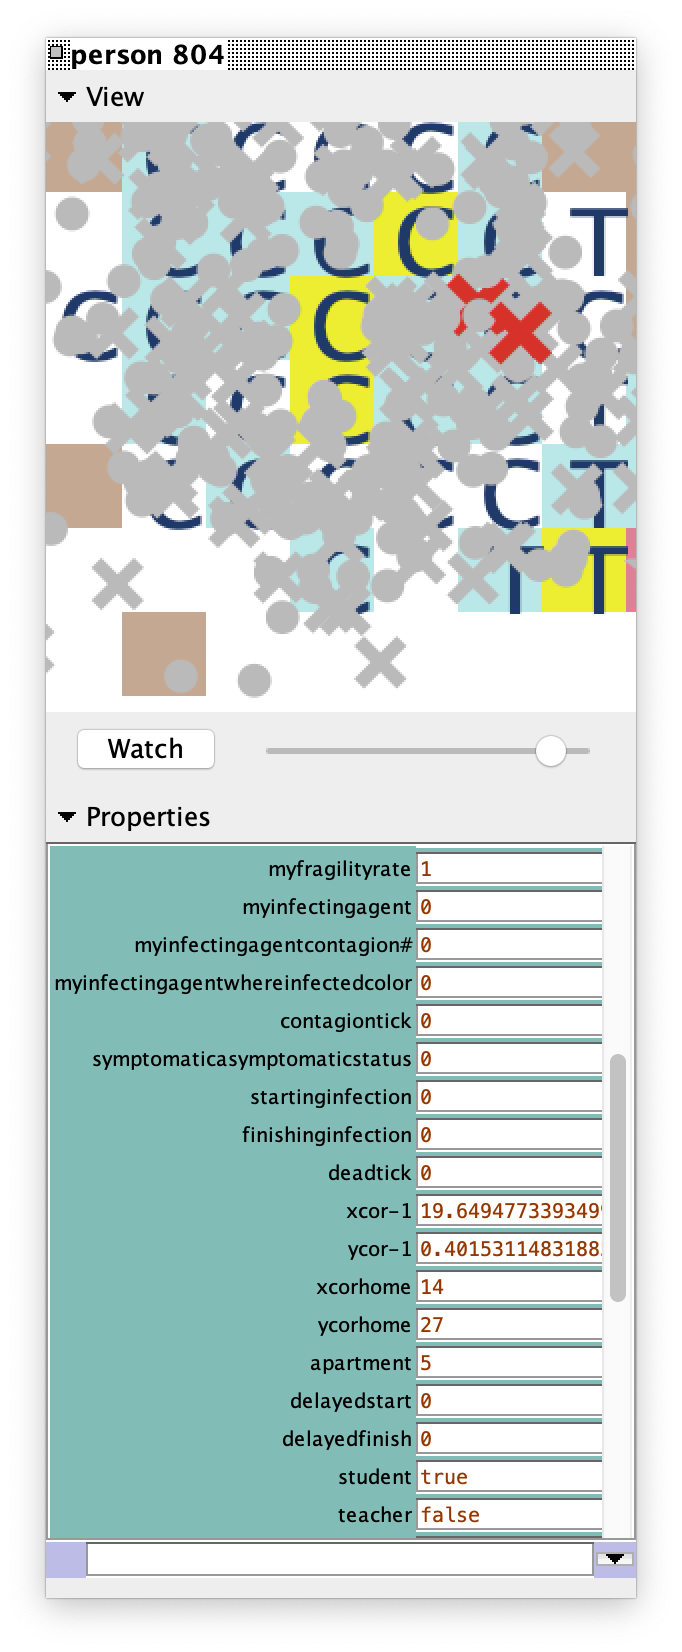
\includegraphics[scale=0.23]{person2.png}

\caption{Probes to different agents} 
\label{diffAgents}
\end{figure}

\end{frame}

%%%%%%%%%%%%%%%%%%%%%%%%%%%%%%%%%%%%%%%%%%%%%%%%%%%%%%%%%
\section{Contagions}

%%%%%%%%%%%%%%%%%%%%%%%%%%%%%%%%%%%%%%%%%%%%%%%%%%%%%%%%%
\subsection{The proposed technique}

%%%%%%%%%%%%%%%%%%%%%%%%%%%%%%%%%%%%%%%%%%%%%%%%%%%%%%%%%
\begin{frame}{Contagion representation}

  \begin{itemize}
  \item
The model allows analyzing the sequences of contagions in simulated epidemics, reporting the places where the contagion occur. 
  \item
We represent each infecting agent as a horizontal segment with a vertical connections to another agent receiving the infection. 
We represent the infected agents via further segments at an upper layer. 

  \item
With colors, line thickness, and styles, we display multiple information. 

  \item
This enables understanding at a glance how an epidemic episode is developing. In this way, it is easier to reason about countermeasures and, thus, to develop intervention policies.

  \end{itemize}
\end{frame}

%%%%%%%%%%%%%%%%%%%%%%%%%%%%%%%%%%%%%%%%%%%%%%%%%%%%%%%%%
\subsection{An introductory example}


%%%%%%%%%%%%%%%%%%%%%%%%%%%%%%%%%%%%%%%%%%%%%%%%%%%%%%%%%
\begin{frame}{An example (1/2)}

\begin{figure}[H]
\center
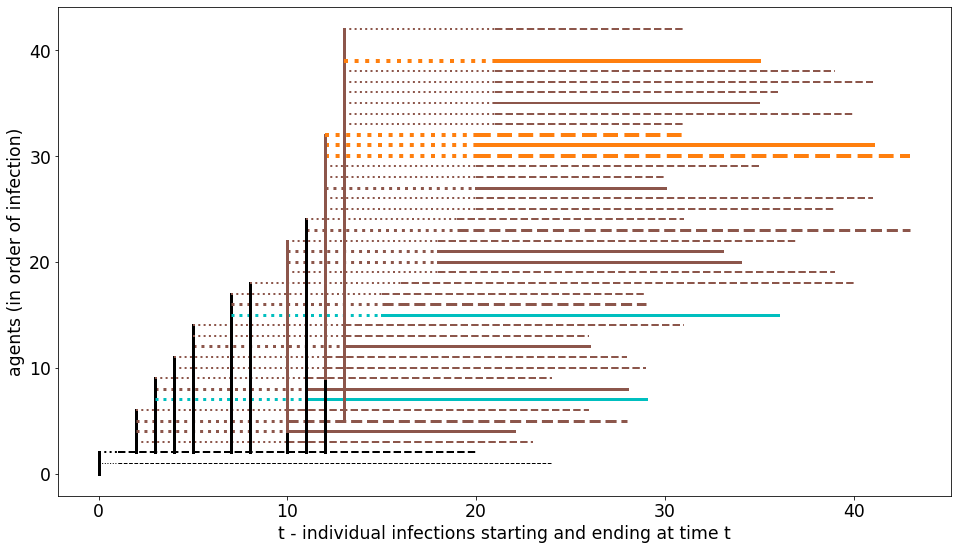
\includegraphics[width=0.9\textwidth]{with8b40.png}% with control case 473323 474697 in SIsaR_0.9.4.1 experiments 2 seeds with control-table_10000.csv, file withControl_473323_474697.csv
\caption{A case with containment measures, first 40 infections: workplaces (brown) and nursing homes (orange) strictly interweaving}
\label{workplacesNursingHomes}
\end{figure}
\end{frame}

%%%%%%%%%%%%%%%%%%%%%%%%%%%%%%%%%%%%%%%%%%%%%%%%%%%%%%%%%
\begin{frame}{An example (2/2), more contagions}

\begin{figure}[H]
\center
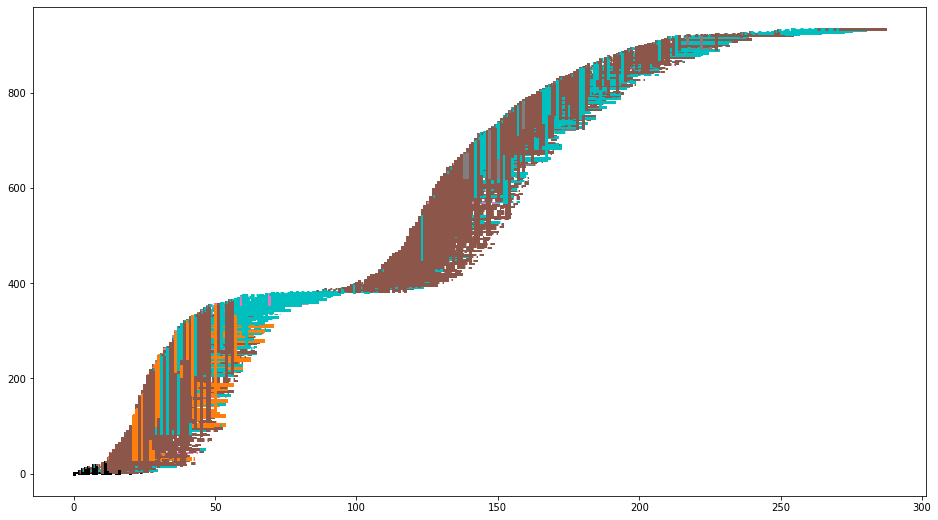
\includegraphics[width=0.9\textwidth]{with8a.png}% with control case 473323 474697 in SIsaR_0.9.4.1 experiments 2 seeds with control-table_10000.csv, file withControl_473323_474697.csv
\caption{A Case with containment measures, the whole epidemics: workplaces (brown) and nursing homes (orange) and then houses (cyan), with a bridge connecting two waves}
\label{workplacesNursingHomes}
\end{figure}


\end{frame}

%%%%%%%%%%%%%%%%%%%%%%%%%%%%%%%%%%%%%%%%%%%%%%%%%%%%%%%%%
\begin{frame}{Other examples (i) on the left, an epidemic without containment measures; (ii) on the right, an epidemic with basic non-pharmaceutical containment measures}

\begin{figure}[H]
\center
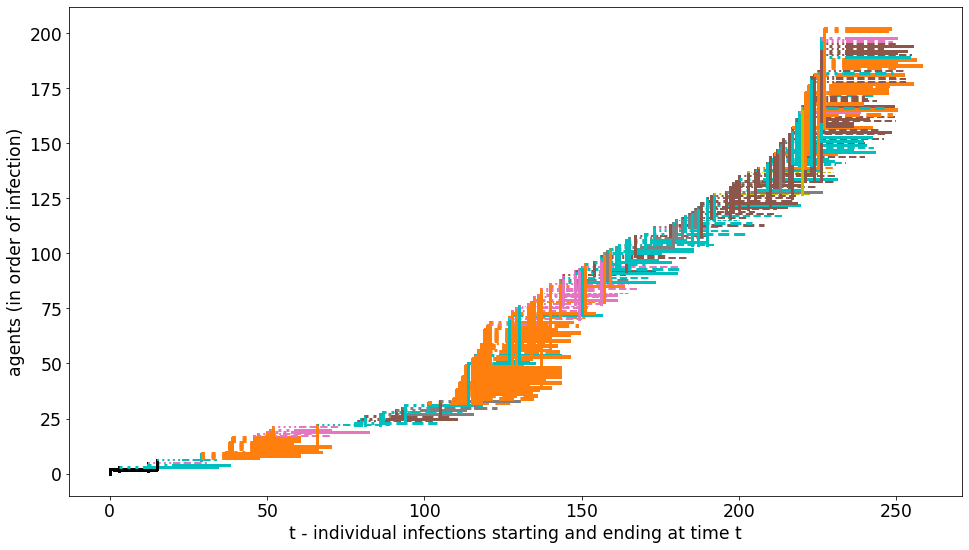
\includegraphics[scale=0.12]{no4b.png}~~~~~~~~~~~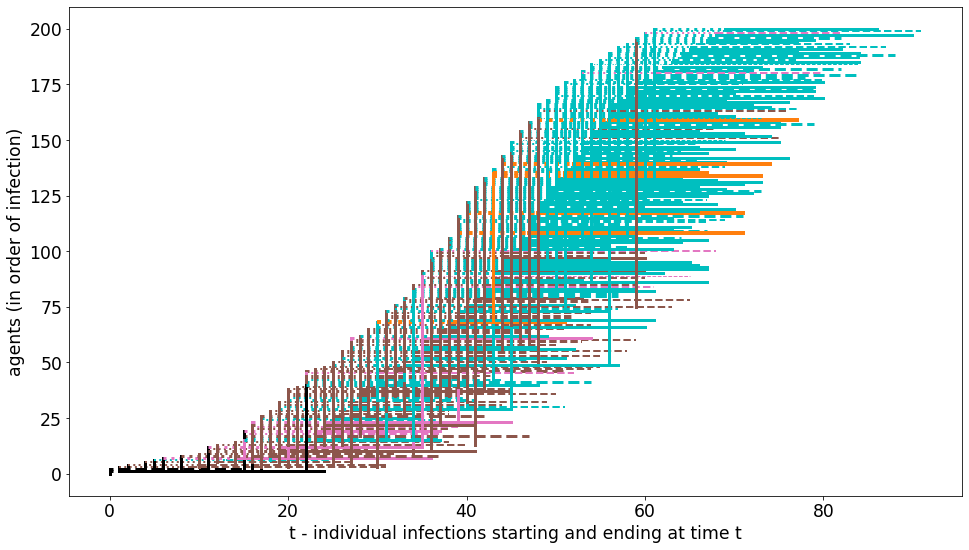
\includegraphics[scale=0.12]{with7b.png} 

\center
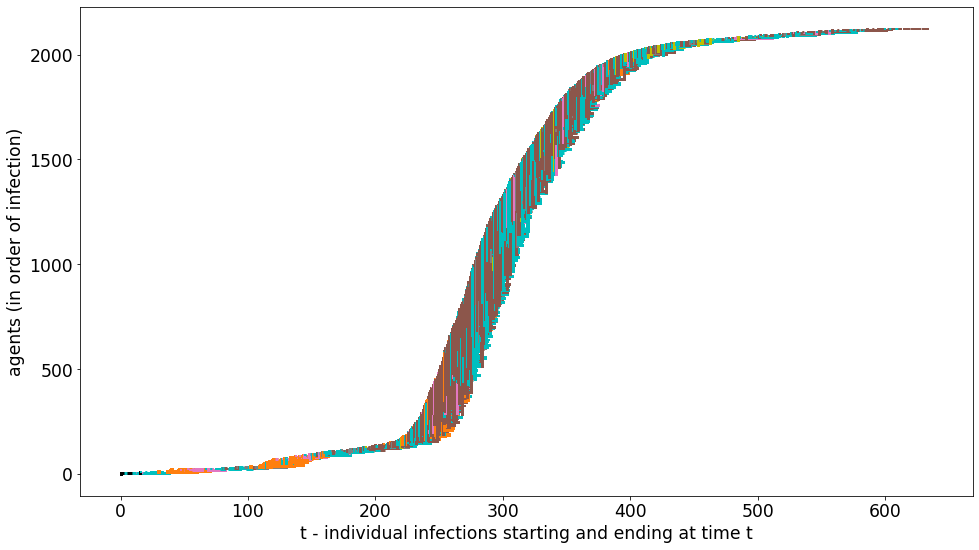
\includegraphics[scale=0.12]{no4a.png}~~~~~~~~~~~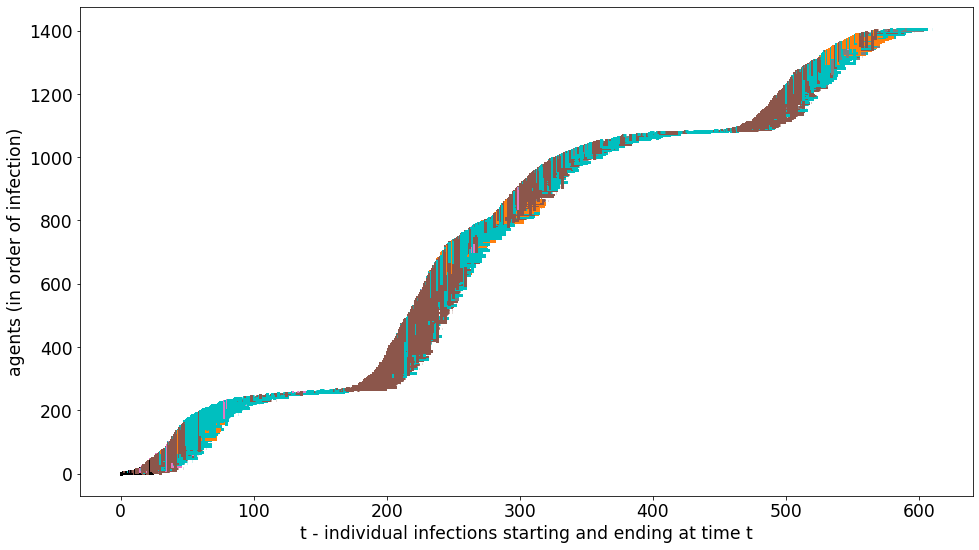
\includegraphics[scale=0.12]{with7a.png} \\
\caption{Two cases with initial and full periods} 
\label{twocases}
\end{figure}

\end{frame}

%%%%%%%%%%%%%%%%%%%%%%%%%%%%%%%%%%%%%%%%%%%%%%%%%%%%%%%%%
\subsection{A significant sequence}

%%%%%%%%%%%%%%%%%%%%%%%%%%%%%%%%%%%%%%%%%%%%%%%%%%%%%%%%%
\begin{frame}{}

A contagion sequence suggesting policies: in Fig. \ref{fourSequences} we can look both at the places where contagions occur and at the dynamics emerging with different levels of intervention. 

\begin{figure}[H]
\center
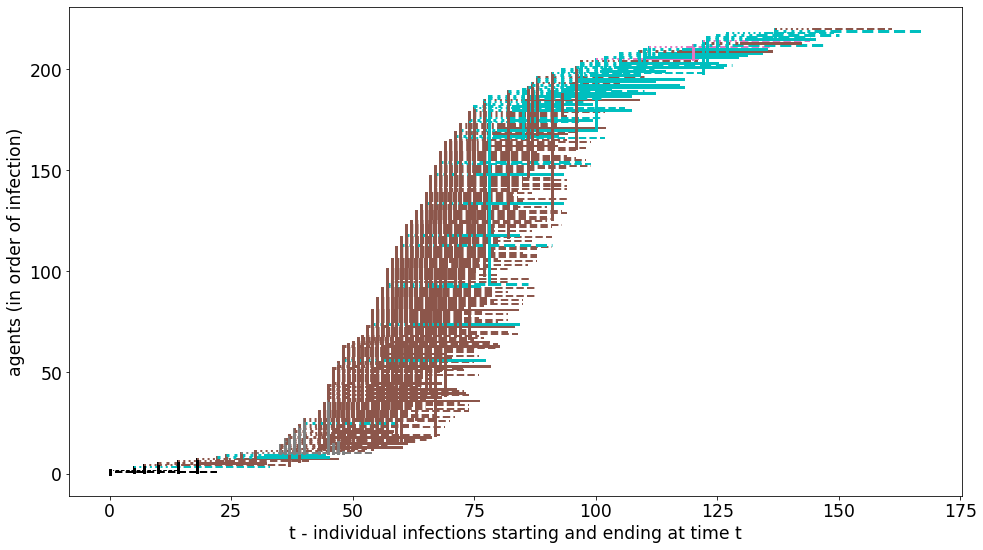
\includegraphics[scale=0.105]{withShort1.png}~~~~~~~~~~~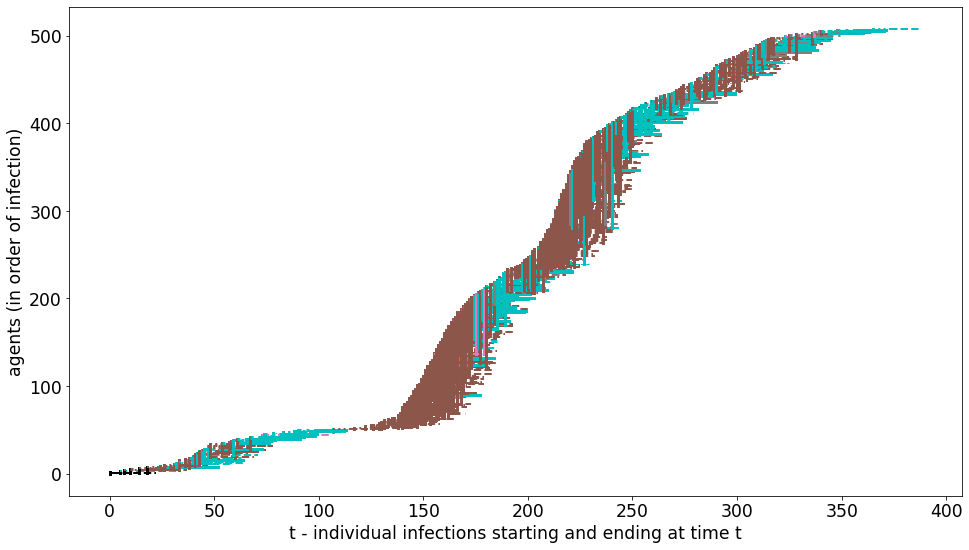
\includegraphics[scale=0.105]{withShort1A.png} 

\center
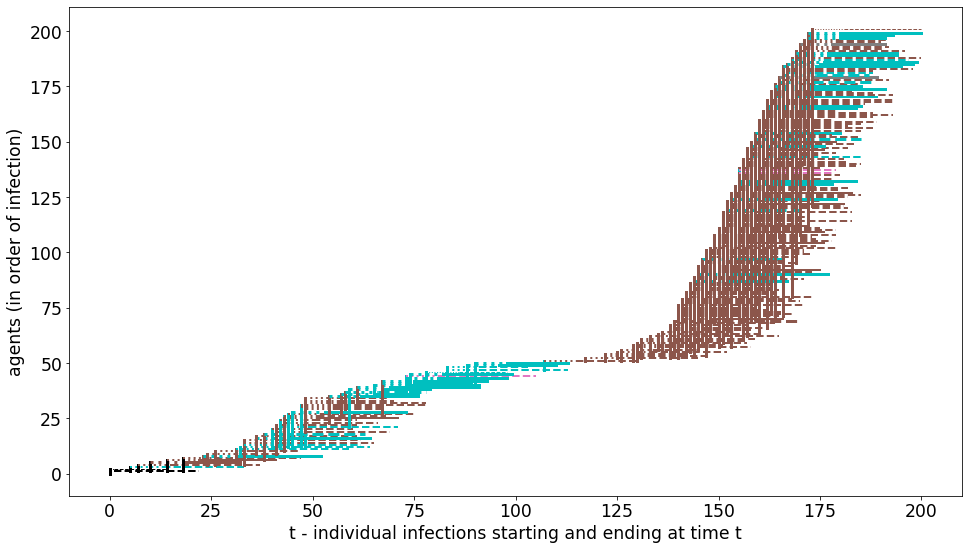
\includegraphics[scale=0.105]{withShort1A200.png}~~~~~~~~~~~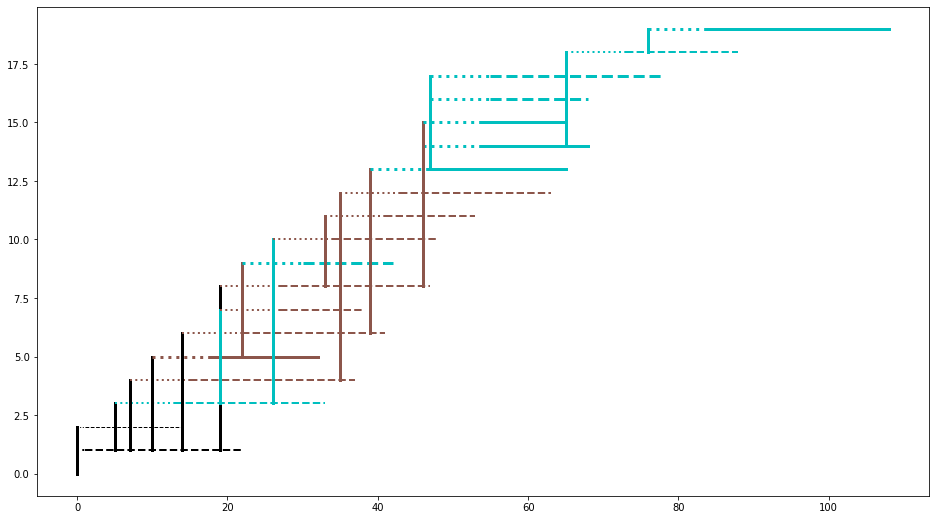
\includegraphics[scale=0.105]{withShort1B.png} \\
\caption{(\emph{top left}) an epidemic with regular containment measures, showing a highly significant effect of workplaces (brown);
 (\emph{top right}) the effects of stopping fragile workers at day 20, with a positive result, but home contagions (cyan) keep alive the pandemic, exploding again in workplaces (brown); (\emph{bottom left}) the same analyzing the first 200 infections with evidence of the event around day 110 with the new phase due to a unique asymptomatic worker, and (\emph{bottom right}) stopping fragile workers and any case of fragility at day 15, also isolating nursing homes} 
\label{fourSequences}
\end{figure}

\end{frame}

%%%%%%%%%%%%%%%%%%%%%%%%%%%%%%%%%%%%%%%%%%%%%%%%%%%%%%%%%
\section{Exploring cases}

%%%%%%%%%%%%%%%%%%%%%%%%%%%%%%%%%%%%%%%%%%%%%%%%%%%%%%%%%
\subsection{Simulation batches}

%%%%%%%%%%%%%%%%%%%%%%%%%%%%%%%%%%%%%%%%%%%%%%%%%%%%%%%%%
\begin{frame}{Simulation batches}

  \begin{itemize}
  \item

We explore systematically the introduction of factual, counterfactual, and prospective interventions to control the spread of the contagions. 

  \item
Each simulation run---whose length coincides with the disappearance of symptomatic or asymptomatic contagion cases---is a datum in a wide scenario of variability in time and effects.   
  
  \item
Consequently, we need to represent compactly the results  emerging from batches of simulation repetitions, to compare the  consequences of the basic assumptions adopted for each specific batch.

 \item
We use blocs of ten thousand repetitions. Besides summarizing the results with the usual statistical indicators, we adopt the technique of the heatmaps.

\item
Each heatmap reports the duration of each simulated epidemic in the $x$ axis and the number of the symptomatic, asymptomatic, and deceased agents in the $y$ axis. The $z$ axis is represented by the colors, in logarithmic scale. 

\item
In our batches we have 10,000 runs.

\end{itemize}
\end{frame}

%%%%%%%%%%%%%%%%%%%%%%%%%%%%%%%%%%%%%%%%%%%%%%%%%%%%%%%%%
\subsection{Epidemics without and with control}

%%%%%%%%%%%%%%%%%%%%%%%%%%%%%%%%%%%%%%%%%%%%%%%%%%%%%%%%%
\begin{frame}{Ten thousand epidemics without control in Piedmont}

% readRunResults10kStableSeedsCPoints_noControl_ChangingWorld_plusHMlog

\begin{table}[H]
\center
\tiny

\begin{tabular}{lrrr}
\toprule
{} &  symptomatic &  totalInfected\&Deceased &  duration \\
\midrule
count &     10000.00 &                10000.00 &  10000.00 \\
mean  &       969.46 &                 2500.45 &    303.10 \\
std   &       308.80 &                  802.88 &     93.50 \\
\bottomrule
\end{tabular}

\label{noCTab}
%\caption{a caption}
\end{table}

\begin{figure}[H]
\center
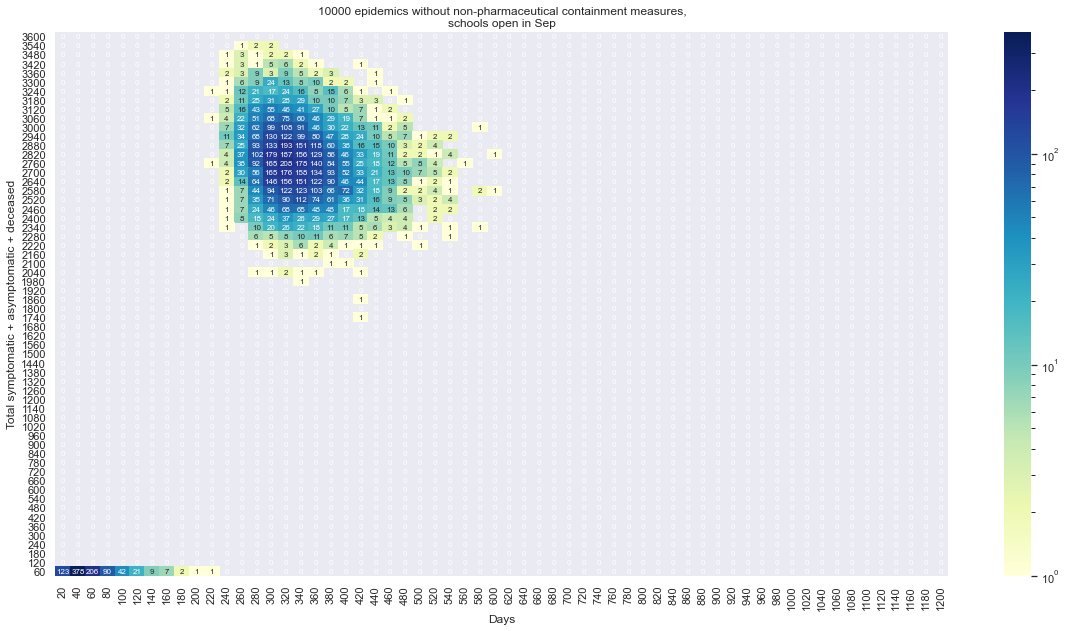
\includegraphics[scale=0.22]{10kNoControl.png}
\caption{Without non-pharmaceutical containment measures} 
\label{noC}
\end{figure}

\end{frame}


%%%%%%%%%%%%%%%%%%%%%%%%%%%%%%%%%%%%%%%%%%%%%%%%%%%%%%%%%
\begin{frame}{Ten thousand epidemics with basic control in Piedmont}

% readRunResults10kStableSeedsCPoints_basicControlB_schoolOpenSeptChangingWorld_plusHMlog

\begin{table}[H]
\center
\tiny

\begin{tabular}{lrrr}
\toprule
{} &  symptomatic &  totalInfected\&Deceased &  duration \\
\midrule
count &     10000.00 &                10000.00 &  10000.00 \\
mean  &       344.22 &                  851.64 &    277.93 \\
std   &       368.49 &                  916.41 &    213.48 \\
\bottomrule
\end{tabular}

\label{basicCTab}
%\caption{a caption}
\end{table}

\begin{figure}[H]
\center
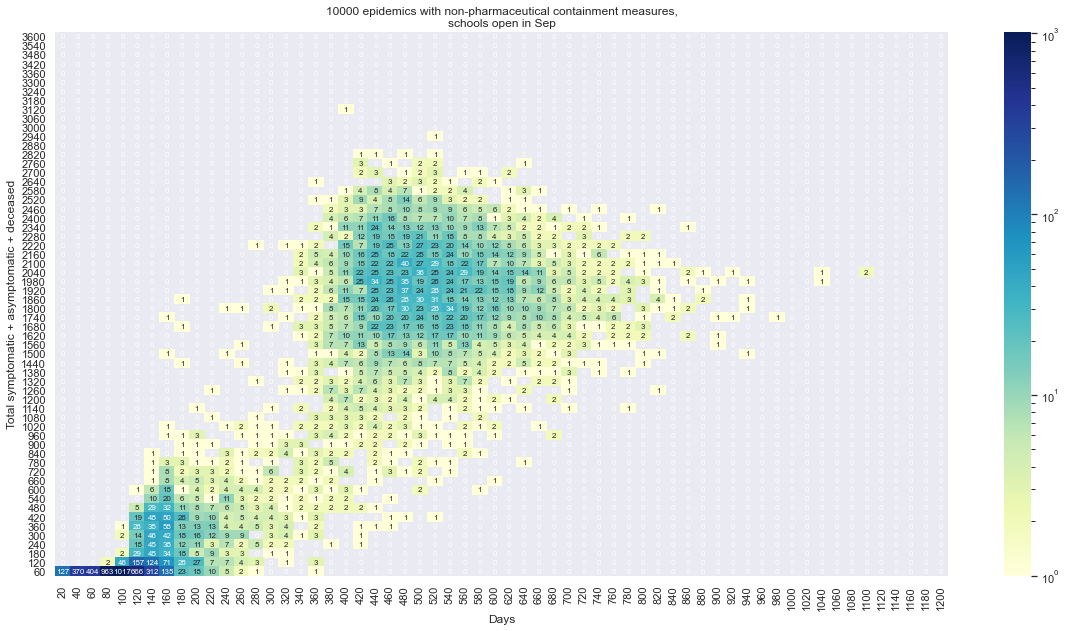
\includegraphics[scale=0.22]{10kBasicC.png}
\caption{First wave with non-pharmaceutical containment measures} 
\label{basicC}
\end{figure}

\end{frame}


%%%%%%%%%%%%%%%%%%%%%%%%%%%%%%%%%%%%%%%%%%%%%%%%%%%%%%%%%
\subsection{Actual data}

%%%%%%%%%%%%%%%%%%%%%%%%%%%%%%%%%%%%%%%%%%%%%%%%%%%%%%%%%
\begin{frame}{Actual data}

\begin{figure}[H]
\center
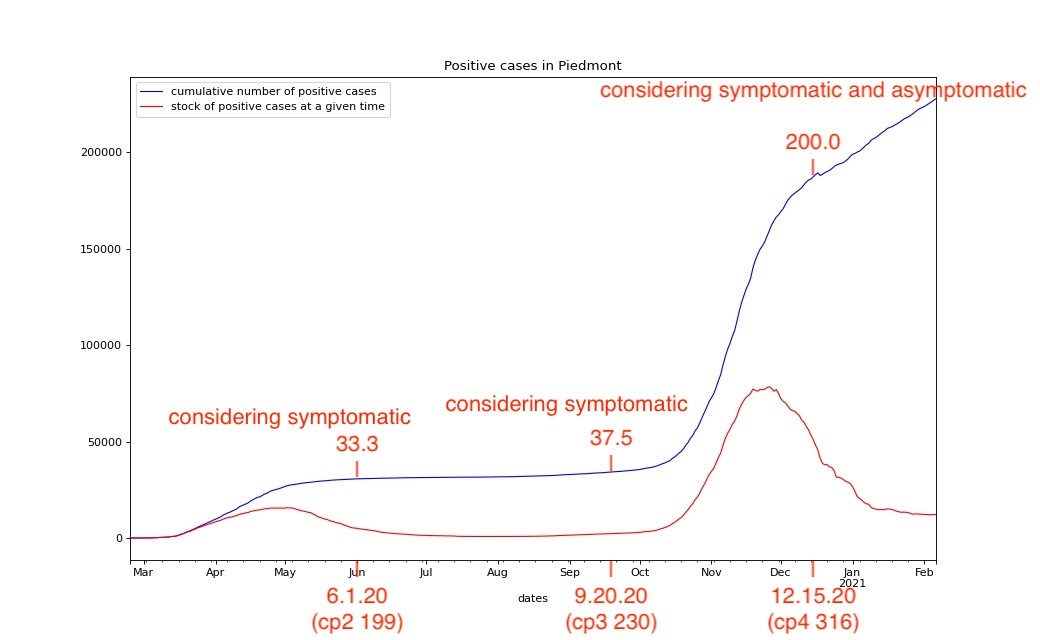
\includegraphics[scale=0.25]{andamento900annotato.jpg}
\caption{Data in Piedmont} 
\label{data}
\end{figure}


\end{frame}



%%%%%%%%%%%%%%%%%%%%%%%%%%%%%%%%%%%%%%%%%%%%%%%%%%%%%%%%%
\subsection{Second wave}

%1%%%%%%%%%%%%%%%%%%%%%%%%%%%%%%%%%%%%%%%%%%%%%%%%%%%%%%%%
\begin{frame}{Spontaneous second wave, without specific measures}

% selectResults10kStableSeedsCPoints_basicControlB_schoolOpenSeptChangingWorld_plusHMlog,ipynb
% using 10kCtrl1.csv from SIsaR_0.9.5.4.1trials10kCtrl1.nlogo

\textbf{170} {\tiny epidemics stable in Summer 2020 out of 10,000, rule: at Jun~1,~20 select if sym. (10, 70], actual v. 33.3 \& at Sep~20,~20 select if sym. (20, 90], actual value 37.5;} \textbf{140} {\tiny at Dec~15,~20, rule: sym.+asym.>Sep~20,~20, actual value: 200.0.}

\begin{figure}[H]
\center
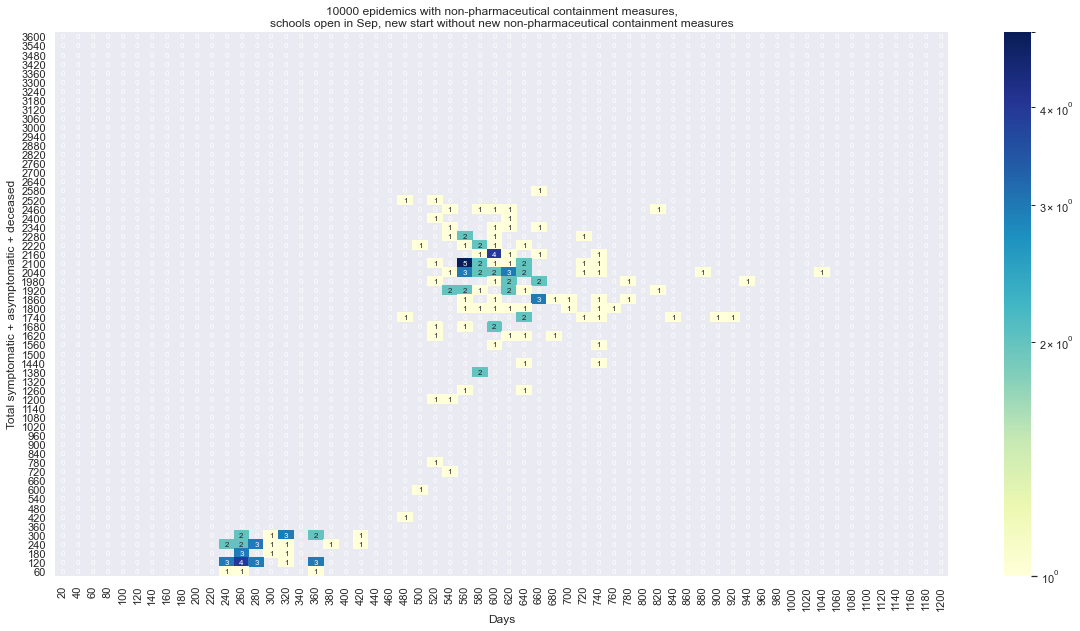
\includegraphics[scale=0.17]{10kSpontWave2.png}
\caption{First wave with non-pharmaceutical containment measures, spontaneous second wave, without specific measures}
\label{selSpontWave2}
\end{figure}

%\vspace{-0.4cm}

\begin{table}[H]
\center
\tiny
\begin{tabular}{p{0.3cm}p{0.3cm}p{0.3cm}p{0.3cm}p{0.3cm}p{0.3cm}p{0.3cm}p{0.3cm}p{0.3cm}p{0.3cm}p{0.3cm}p{0.3cm}p{0.3cm}p{0.4cm}}
\toprule
(1000) &  Jun~1,~20 & &  Sep~9,~20 & & Dec~15,~20 & & Feb~1,~21 & & May~1,~21 & & Dec~15,~20~~~to~~~end  \\
{} &  sym. &  all &  sympt. &  totalInf. &  sympt. &  totalInf. &  sympt. &  totalInf. &  sympt. &  totalInf. &  sympt. &  totalInf.  & days\\
\midrule
count &    170.0 &                      170.0 &    170.0 &                      170.0 &    140.0 &                      140.0 &    131.0 &                      131.0 &    128.0 &                      128.0 &               140.0 &                   140.0 &  140.0 \\
mean  &     37.9 &                      100.2 &     60.4 &                      159.3 &    \textbf{248.4} &                      \textbf{648.7} &    \textbf{432.2} &                     \textbf{1109.5} &   \textbf{656.3} &                     \textbf{1655.5} &              701.1 &                  1757.9 &  594.2 \\
std   &     16.4 &                       61.0 &     19.6 &                       71.7 &    167.4 &                      424.3 &    220.4 &                      538.4 &    215.4 &                      513.3 &               246.4 &                   599.7 &  118.9 \\
\bottomrule
\end{tabular}

\label{selSpontWave2Tab}
%\caption{a caption}
\end{table}


\end{frame}

%2%%%%%%%%%%%%%%%%%%%%%%%%%%%%%%%%%%%%%%%%%%%%%%%%%%%%%%%%
\begin{frame}{Second w., new infections from outside, without specific measures}

% selectResults10kStableSeedsCPoints_basicControlB_schoolOpenSeptChangingWorldNewStart_plusHMlog.ipynb
% using 10kCtrl1NStart.csv from SIsaR_0.9.5.4.1trials10kCtrl1NStart.nlogo

\textbf{1407} {\tiny epidemics stable in Summer 2020 out of 10,000, rule: at Jun~1,~20 select if sym. (10, 70], actual v. 33.3 \& at Sep~20,~20 select if sym. (20, 90], actual value 37.5;} \textbf{1044} {\tiny at Dec~15,~20, rule: sym.+asym.>Sep~20,~20, actual value: 200.0.}

\begin{figure}[H]
\center
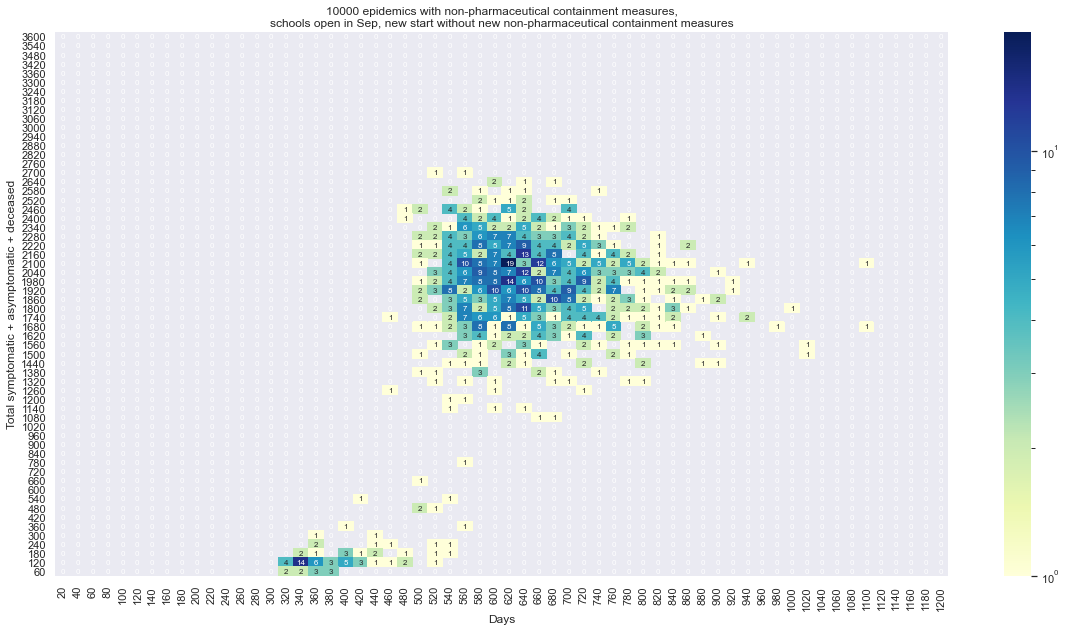
\includegraphics[scale=0.17]{10kForceWave2.png}
\caption{First wave with non-pharmaceutical containment measures, forcing the second wave, without specific measures}
\label{selForceWave2}
\end{figure}

%\vspace{-0.4cm}

\begin{table}[H]
\center
\tiny
\begin{tabular}{p{0.3cm}p{0.3cm}p{0.3cm}p{0.3cm}p{0.3cm}p{0.3cm}p{0.3cm}p{0.3cm}p{0.3cm}p{0.3cm}p{0.3cm}p{0.3cm}p{0.3cm}p{0.4cm}}
\toprule
(1000) &  Jun~1,~20 & &  Sep~9,~20 & & Dec~15,~20 & & Feb~1,~21 & & May~1,~21 & & Dec~15,~20~~~to~~~end   \\
{} &  sym. &  all &  sympt. &  totalInf. &  sympt. &  totalInf. &  sympt. &  totalInf. &  sympt. &  totalInf. &  sympt. &  totalInf.  & days\\
\midrule
count &   1407.0 &                     1407.0 &   1407.0 &                     1407.0 &   1044.0 &                     1044.0 &   1005.0 &                     1005.0 &    980.0 &                      980.0 &              1044.0 &                  1044.0 & 1044.0 \\
mean  &     35.6 &                       72.7 &     40.0 &                       84.1 &    \textbf{180.4} &                      \textbf{462.1} &    \textbf{354.1} &                      \textbf{900.4} &    \textbf{623.8} &                     \textbf{1563.3} &               726.6 &                  1810.9 &  620.9 \\
std   &     14.1 &                       42.6 &     16.7 &                       52.8 &    134.6 &                      354.6 &    213.8 &                      535.4 &    217.9 &                      527.0 &               221.9 &                   544.0 &  110.8 \\
\bottomrule
\end{tabular}

\label{selForceWave2Tab}
%\caption{a caption}
\end{table}


\end{frame}

%3%%%%%%%%%%%%%%%%%%%%%%%%%%%%%%%%%%%%%%%%%%%%%%%%%%%%%%%%
\begin{frame}{Second w., new infections from outside, with new specific measures}

% selectResults10kStableSeedsCPoints_basicControlB_schoolOpenSeptOctMarControlChangingWorldNewStart_plusHMlog.ipynb
% using 10kCtrl1NStartCtrl2M.csv from SIsaR_0.9.5.4.1trials10kCtrl1NStartCtrl2M.nlogo

\textbf{1407} {\tiny epidemics stable in Summer 2020 out of 10,000, rule: at Jun~1,~20 select if sym. (10, 70], actual v. 33.3 \& at Sep~20,~20 select if sym. (20, 90], actual value 37.5;} \textbf{874} {\tiny at Dec~15,~20, rule: sym.+asym.>Sep~20,~20, actual value: 200.0.}

\begin{figure}[H]
\center
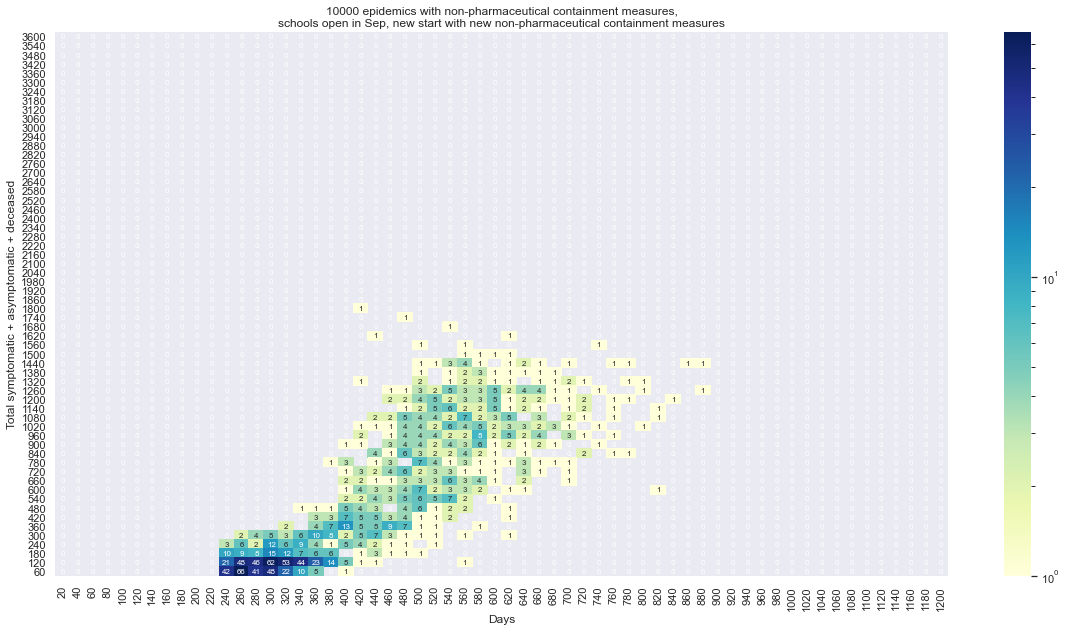
\includegraphics[scale=0.17]{10kForceWave2Contr2.png}
\caption{First wave with non-ph.containment measures, forcing the second wave, \textbf{with new specific non-ph. containment measures}}
\label{selForceWave2Contr2}
\end{figure}

%\vspace{-0.4cm}

\begin{table}[H]
\center
\tiny
\begin{tabular}{p{0.3cm}p{0.3cm}p{0.3cm}p{0.3cm}p{0.3cm}p{0.3cm}p{0.3cm}p{0.3cm}p{0.3cm}p{0.3cm}p{0.3cm}p{0.3cm}p{0.3cm}p{0.4cm}}
\toprule
(1000) &  Jun~1,~20 & &  Sep~9,~20 & & Dec~15,~20 & & Feb~1,~21 & & May~1,~21 & & Dec~15,~20~~~to~~~end   \\
{} &  sym. &  all &  sympt. &  totalInf. &  sympt. &  totalInf. &  sympt. &  totalInf. &  sympt. &  totalInf. &  sympt. &  totalInf.  & days\\
\midrule
count &   1407.0 &                     1407.0 &   1407.0 &                     1407.0 &    874.0 &                      874.0 &    719.0 &                      719.0 &    523.0 &                      523.0 &              874.0 &                   874.0 &  874.0 \\
mean  &     35.6 &                       72.7 &     40.0 &                       84.1 &    \textbf{130.0} &                      \textbf{340}.6 &    \textbf{194.4} &                      \textbf{512.8} &    \textbf{295.7} &                      \textbf{791.2} &               252.7 &                   666.4 &  494.1 \\
std   &     14.1 &                       42.6 &     16.7 &                       52.8 &     83.9 &                      232.6 &    104.1 &                      276.9 &    119.1 &                      300.6 &               156.8 &                   416.4 &  122.7 \\
\bottomrule
\end{tabular}

\label{selSpontWave2Contr2Tab}
%\caption{a caption}
\end{table}


\end{frame}

%4%%%%%%%%%%%%%%%%%%%%%%%%%%%%%%%%%%%%%%%%%%%%%%%%%%%%%%%%
\begin{frame}{Second w., new infect. from outside, with new specific meas. -20 days\footnote{Anticipation limit Oct 5.}}

% selectResults10kStableSeedsCPoints_basicControlB_schoolOpenSeptOctMar-20ControlChangingWorldNewStart_plusHMlog.ipynb
% using 10kCtrl1NStartCtrl2M-20.csv from SIsaR_0.9.5.4.1trials10kCtrl1NStartCtrl2M-20.nlogo

\textbf{1407} {\tiny epidemics stable in Summer 2020 out of 10,000, rule: at Jun~1,~20 select if sym. (10, 70], actual v. 33.3 \& at Sep~20,~20 select if sym. (20, 90], actual value 37.5;} \textbf{769} {\tiny at Dec~15,~20, rule: sym.+asym.>Sep~20,~20, actual value: 200.0.}

\begin{figure}[H]
\center
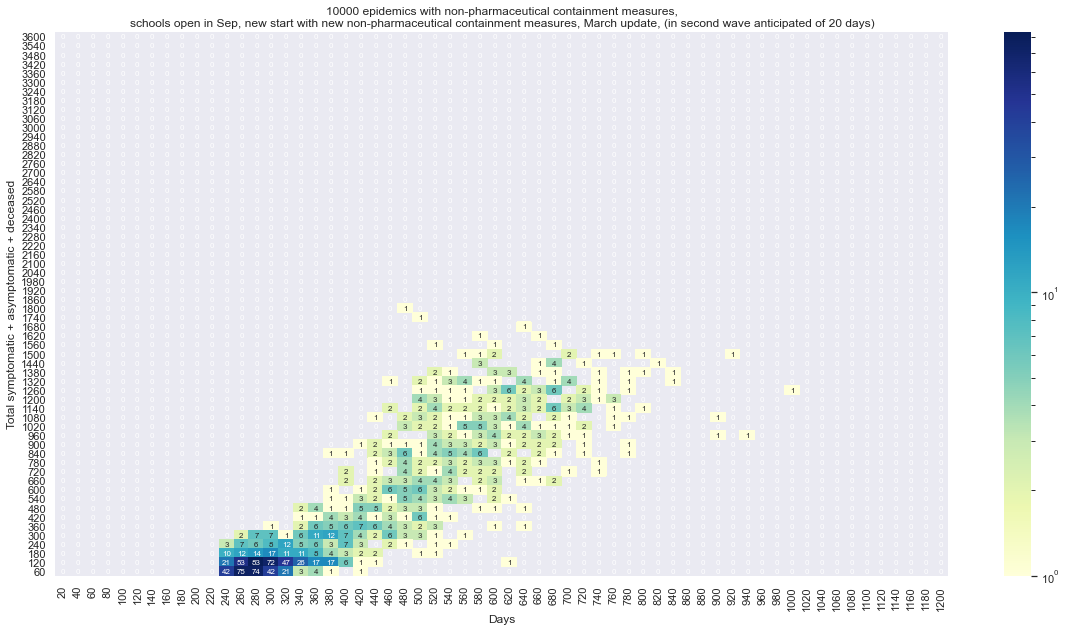
\includegraphics[scale=0.17]{10kForceWave2Contr2M-20.png}
\caption{First wave with non-ph.cont. meas., forcing the second wave, \textbf{with new specific non-ph. cont. meas., 20 day anticipation}}
\label{selForceWave2Contr2M-20}
\end{figure}

%\vspace{-0.4cm}

\begin{table}[H]
\center
\tiny
\begin{tabular}{p{0.3cm}p{0.3cm}p{0.3cm}p{0.3cm}p{0.3cm}p{0.3cm}p{0.3cm}p{0.3cm}p{0.3cm}p{0.3cm}p{0.3cm}p{0.3cm}p{0.3cm}p{0.4cm}}
\toprule
(1000) &  Jun~1,~20 & &  Sep~9,~20 & & Dec~15,~20 & & Feb~1,~21 & & May~1,~21 & & Dec~15,~20~~~to~~~end   \\
{} &  sym. &  all &  sympt. &  totalInf. &  sympt. &  totalInf. &  sympt. &  totalInf. &  sympt. &  totalInf. &  sympt. &  totalInf.  & days\\
\midrule
count &   1407.0 &                     1407.0 &   1407.0 &                     1407.0 &    769.0 &                      769.0 &    637.0 &                      637.0 &    471.0 &                      471.0 &              769.0 &                   769.0 &  769.0 \\
mean  &     35.6 &                       72.7 &     40.0 &                       84.1 &    \textbf{{\color{red}112.2}} &                     \textbf{{\color{red} 294.2}} &    \textbf{172.0} &                      \textbf{467.9} &    \textbf{276.5} &                      \textbf{748.6} &              248.9 &                   663.4 &  499.3 \\
std   &     14.1 &                       42.6 &     16.7 &                       52.8 &     66.8 &                      188.4 &     91.5 &                      251.3 &    112.9 &                      286.9 &               158.0 &                   417.5 &  124.1 \\
\bottomrule
\end{tabular}

\label{selForceWave2Contr2M-20Tab}
%\caption{a caption}
\end{table}


\end{frame}


%5%%%%%%%%%%%%%%%%%%%%%%%%%%%%%%%%%%%%%%%%%%%%%%%%%%%%%%%%
\begin{frame}{Sec. w., new infect. from outs., stop fragile people. 60  days from Oct. 5\footnote{Schools are always working 100\% in this case.}}

%selectResults10kStableSeedsCPoints_basicControlB_schoolOpenSeptNoFragOCT05-60dControlChangingWorldNewStart_plusHMlog.ipynb
% using 10kCtrl1NStartNoFragOCT05-60d.csv from SIsaR_0.9.5.4.1trials10kCtrl1NStartNoFragOCT05-60d.nlogo

\textbf{1407} {\tiny epidemics stable in Summer 2020 out of 10,000, rule: at Jun~1,~20 select if sym. (10, 70], actual v. 33.3 \& at Sep~20,~20 select if sym. (20, 90], actual value 37.5;} \textbf{886} {\tiny at Dec~15,~20, rule: sym.+asym.>Sep~20,~20, actual value: 200.0.}

\begin{figure}[H]
\center
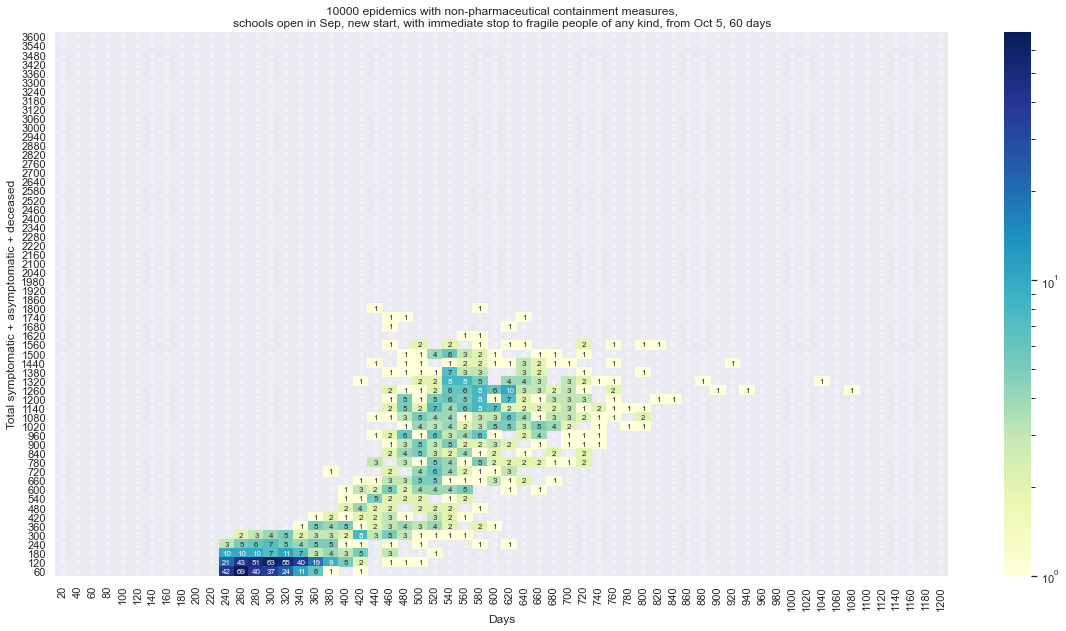
\includegraphics[scale=0.17]{10kForceWave2NoFragOct5for60d.png}
\caption{First wave with non-ph, cont, meas., forcing the sec. w.; \textbf{in sec. w., uniquely stop fragile people, including fragile workers}} 
\label{selForceWave2NoFrag}
\end{figure}

%\vspace{-0.4cm} 

\begin{table}[H]
\center
\tiny
\begin{tabular}{p{0.3cm}p{0.3cm}p{0.3cm}p{0.3cm}p{0.3cm}p{0.3cm}p{0.3cm}p{0.3cm}p{0.3cm}p{0.3cm}p{0.3cm}p{0.3cm}p{0.3cm}p{0.4cm}}
\toprule
(1000) &  Jun~1,~20 & &  Sep~9,~20 & & Dec~15,~20 & & Feb~1,~21 & & May~1,~21 & & Dec~15,~20~~~to~~~end   \\
{} &  sym. &  all &  sympt. &  totalInf. &  sympt. &  totalInf. &  sympt. &  totalInf. &  sympt. &  totalInf. &  sympt. &  totalInf.  & days\\
\midrule
count &   1407.0 &                     1407.0 &   1407.0 &                     1407.0 &    886.0 &                      886.0 &    761.0 &                      761.0 &    637.0 &                      637.0 &              886.0 &                   886.0 &  886.0 \\
mean  &     35.6 &                       72.7 &     40.0 &                       84.1 &    \textbf{{\color{cyan}128.1}} &                      \textbf{{\color{cyan}326.3}} &    \textbf{211.0} &                      \textbf{555.1} &    \textbf{323.3} &                      \textbf{862.1} &               301.1 &                   792.3 &  515.5 \\
std   &     14.1 &                       42.6 &     16.7 &                       52.8 &     89.6 &                      234.2 &    118.1 &                      306.7 &    126.4 &                      315.9 &               170.7 &                   450.2 &  116.9 \\
\bottomrule
\end{tabular}

\label{selForceWave2NoFragTab}
%\caption{a caption}
\end{table}


\end{frame}




%%%%%%%%%%%%%%%%%%%%%%%%%%%%%%%%%%%%%%%%%%%%%%%%%%%%%%%%%
\begin{frame}{To recap}

\begin{table}[H]
\center
\footnotesize
\begin{tabular}{p{1.8cm}p{0.5cm}p{0.5cm}p{0.5cm}p{0.5cm}p{0.5cm}p{0.5cm}}
\toprule
Scenarios     &    &  Dec~15,~20 &               & Dec~15,~20~~~to~~~end  &  &\\
                     &    & sympt.           &  totalInf. &  sympt. &  totalInf.  & days   \\                               

\midrule
no \\
containments in   & count & 140.0 &                      140.0 &                140.0 &                   140.0 &  140.0 \\
spontaneous         &  mean  &  \textbf{248.4} &                      \textbf{648.7} &      701.1 &                  1757.9 &  594.2 \\
second wave         & std  &  167.4 &                      424.3 &               246.4 &                   599.7 &  118.9 \\

\midrule
no \\
containments in   & count &     1044.0 &                     1044.0 &             1044.0 &                  1044.0 & 1044.0 \\
forced         & mean  &       \textbf{180.4} &                      \textbf{462.1} &          726.6 &                  1810.9 &  620.9 \\
second wave         & std   & 134.6 &                      354.6 &           221.9 &                   544.0 &  110.8 \\

\midrule
basic \\
containements in   & count &     874.0 &                      874.0 &          874.0 &                   874.0 &  874.0 \\
forced                    & mean  &             \textbf{130.0} &                      \textbf{340}.6 &                 252.7 &                   666.4 &  494.1 \\
second wave         & std   &   83.9 &                      232.6 &                  156.8 &                   416.4 &  122.7 \\
         
\midrule
-20 days \\ 
containments in   & count &  769.0 &                      769.0 &               769.0 &                   769.0 &  769.0 \\
forced             & mean  &   \textbf{{\color{red}112.2}} &        \textbf{{\color{red} 294.2}} &       248.9 &        663.4 &  499.3 \\
second wave  & std   &   66.8 &                      188.4 &          158.0 &                   417.5 &  124.1 \\

\midrule
frag. p. \& workers \\  
control in              & count &   886.0 &                      886.0 &              886.0 &                   886.0 &  886.0 \\
forced                  & mean  &  \textbf{{\color{cyan}128.1}} &         \textbf{{\color{cyan}326.3}} &          301.1 &        792.3 &  515.5 \\
second wave       & std   &  89.6 &        234.2 &   170.7 &          450.2 &  116.9 \\


\bottomrule
\end{tabular}
\caption{Report of the key results, with count, mean, and std}
\label{keyResultsT}
\end{table}



\end{frame}

%%%%%%%%%%%%%%%%%%%%%%%%%%%%%%%%%%%%%%%%%%%%%%%%%%%%%%%%%
\section{New use cases of the model}

%%%%%%%%%%%%%%%%%%%%%%%%%%%%%%%%%%%%%%%%%%%%%%%%%%%%%%%%%
\begin{frame}{Exploring vaccinations}

Exploring vaccination sequences (using \emph{genetic algorithms} or \emph{reinforcement learning}).

\end{frame}


%%%%%%%%%%%%%%%%%%%%%%%%%%%%%%%%%%%%%%%%%%%%%%%%%%%%%%%%%
\section{A new model}

%%%%%%%%%%%%%%%%%%%%%%%%%%%%%%%%%%%%%%%%%%%%%%%%%%%%%%%%%
\begin{frame}{A new model: the map}

\begin{figure}[H]
\center
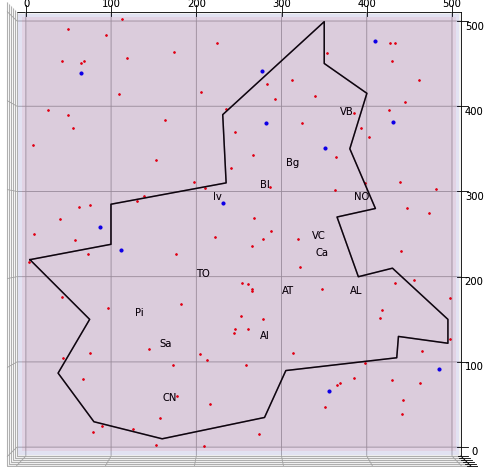
\includegraphics[scale=0.25]{Piem1.png}~~~~~~~~~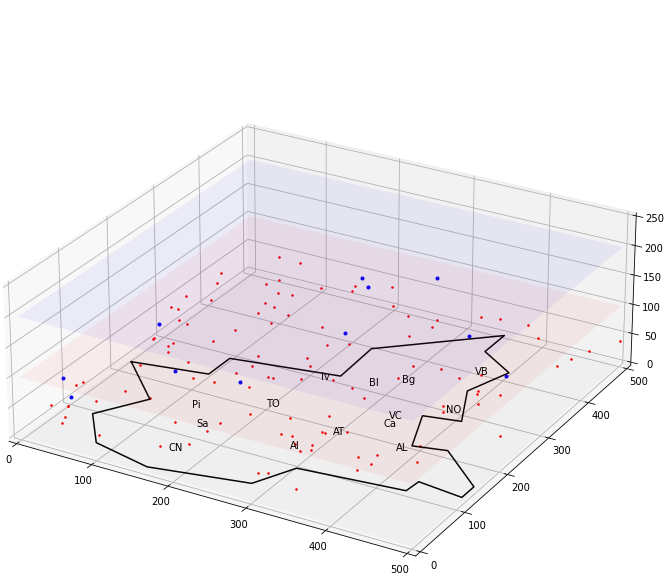
\includegraphics[scale=0.25]{Piem2.png} 

\caption{3D Piedmont} 
\label{Piem}
\end{figure}

\end{frame}

%%%%%%%%%%%%%%%%%%%%%%%%%%%%%%%%%%%%%%%%%%%%%%%%%%%%%%%%%
\begin{frame}{A new model: the scale and the items}

\begin{itemize}

\item $1:100$.

\item \textit{Infection engine}, \url{https://terna.to.it/simul/InfectionEngine.pdf}.

\item Houses.
\item Schools.
\item Hospitals.
\item Nursing homes,
\item Factories.
\color{red}
\item Transportations.
\item Aggregation places: happy hours, night life, sport stadiums, discotheques, \ldots

\end{itemize}

\end{frame}

%%%%%%%%%%%%%%%%%%%%%%%%%%%%%%%%%%%%%%%%%%%%%%%%%%%%%%%%%
\begin{frame}{The tool: S.L.A.P.P.}

Scientific advertising: \url{https://terna.github.io/SLAPP/}

\begin{figure}[H]
\center

\includegraphics[scale=0.26]{SLAPP.png}

\caption{Swarm-Like Agent Protocol in Python} 
\label{SLAPP}
\end{figure}

\end{frame}
%%%%%%%%%%%%%%%%%%%%%%%%%%%%%%%%%%%%%%%%%%%%%%%%%%%%%%%%%
\section{Final remarks}

%%%%%%%%%%%%%%%%%%%%%%%%%%%%%%%%%%%%%%%%%%%%%%%%%%%%%%%%%
\begin{frame}{A few considerations:}

\begin{itemize}

\item
The importance of High Performance Computing.

\item
From S.I.s.a.R. to a model of the society and of the economy of Piedmont.

\bigskip

\item The S.I.s.a.R. model is a tool for comparative analyses, not for forecasting (the enormous standard deviation values are intrinsic to the problem).


\item The model is highly parametric and more it will be.

\item New crisis calling for immediate simulation could take a substantial advantage from the parametric structure of the model.

\end{itemize}

 \bigskip
 The slides are at \url{https://terna.to.it/simul/TernaIRES20210223.pdf}.
 
 My homepage \url{https://terna.to.it} and my address \url{pietro.terna@unito.it}.
 
\end{frame}

%%%%%%%%%%%%%%%%%%%%%%%%%%%%%%%%%%%%%%%%%%%%%%%%%%%%%%%%%
\begin{frame}{}

\begin{figure}[H]
\center
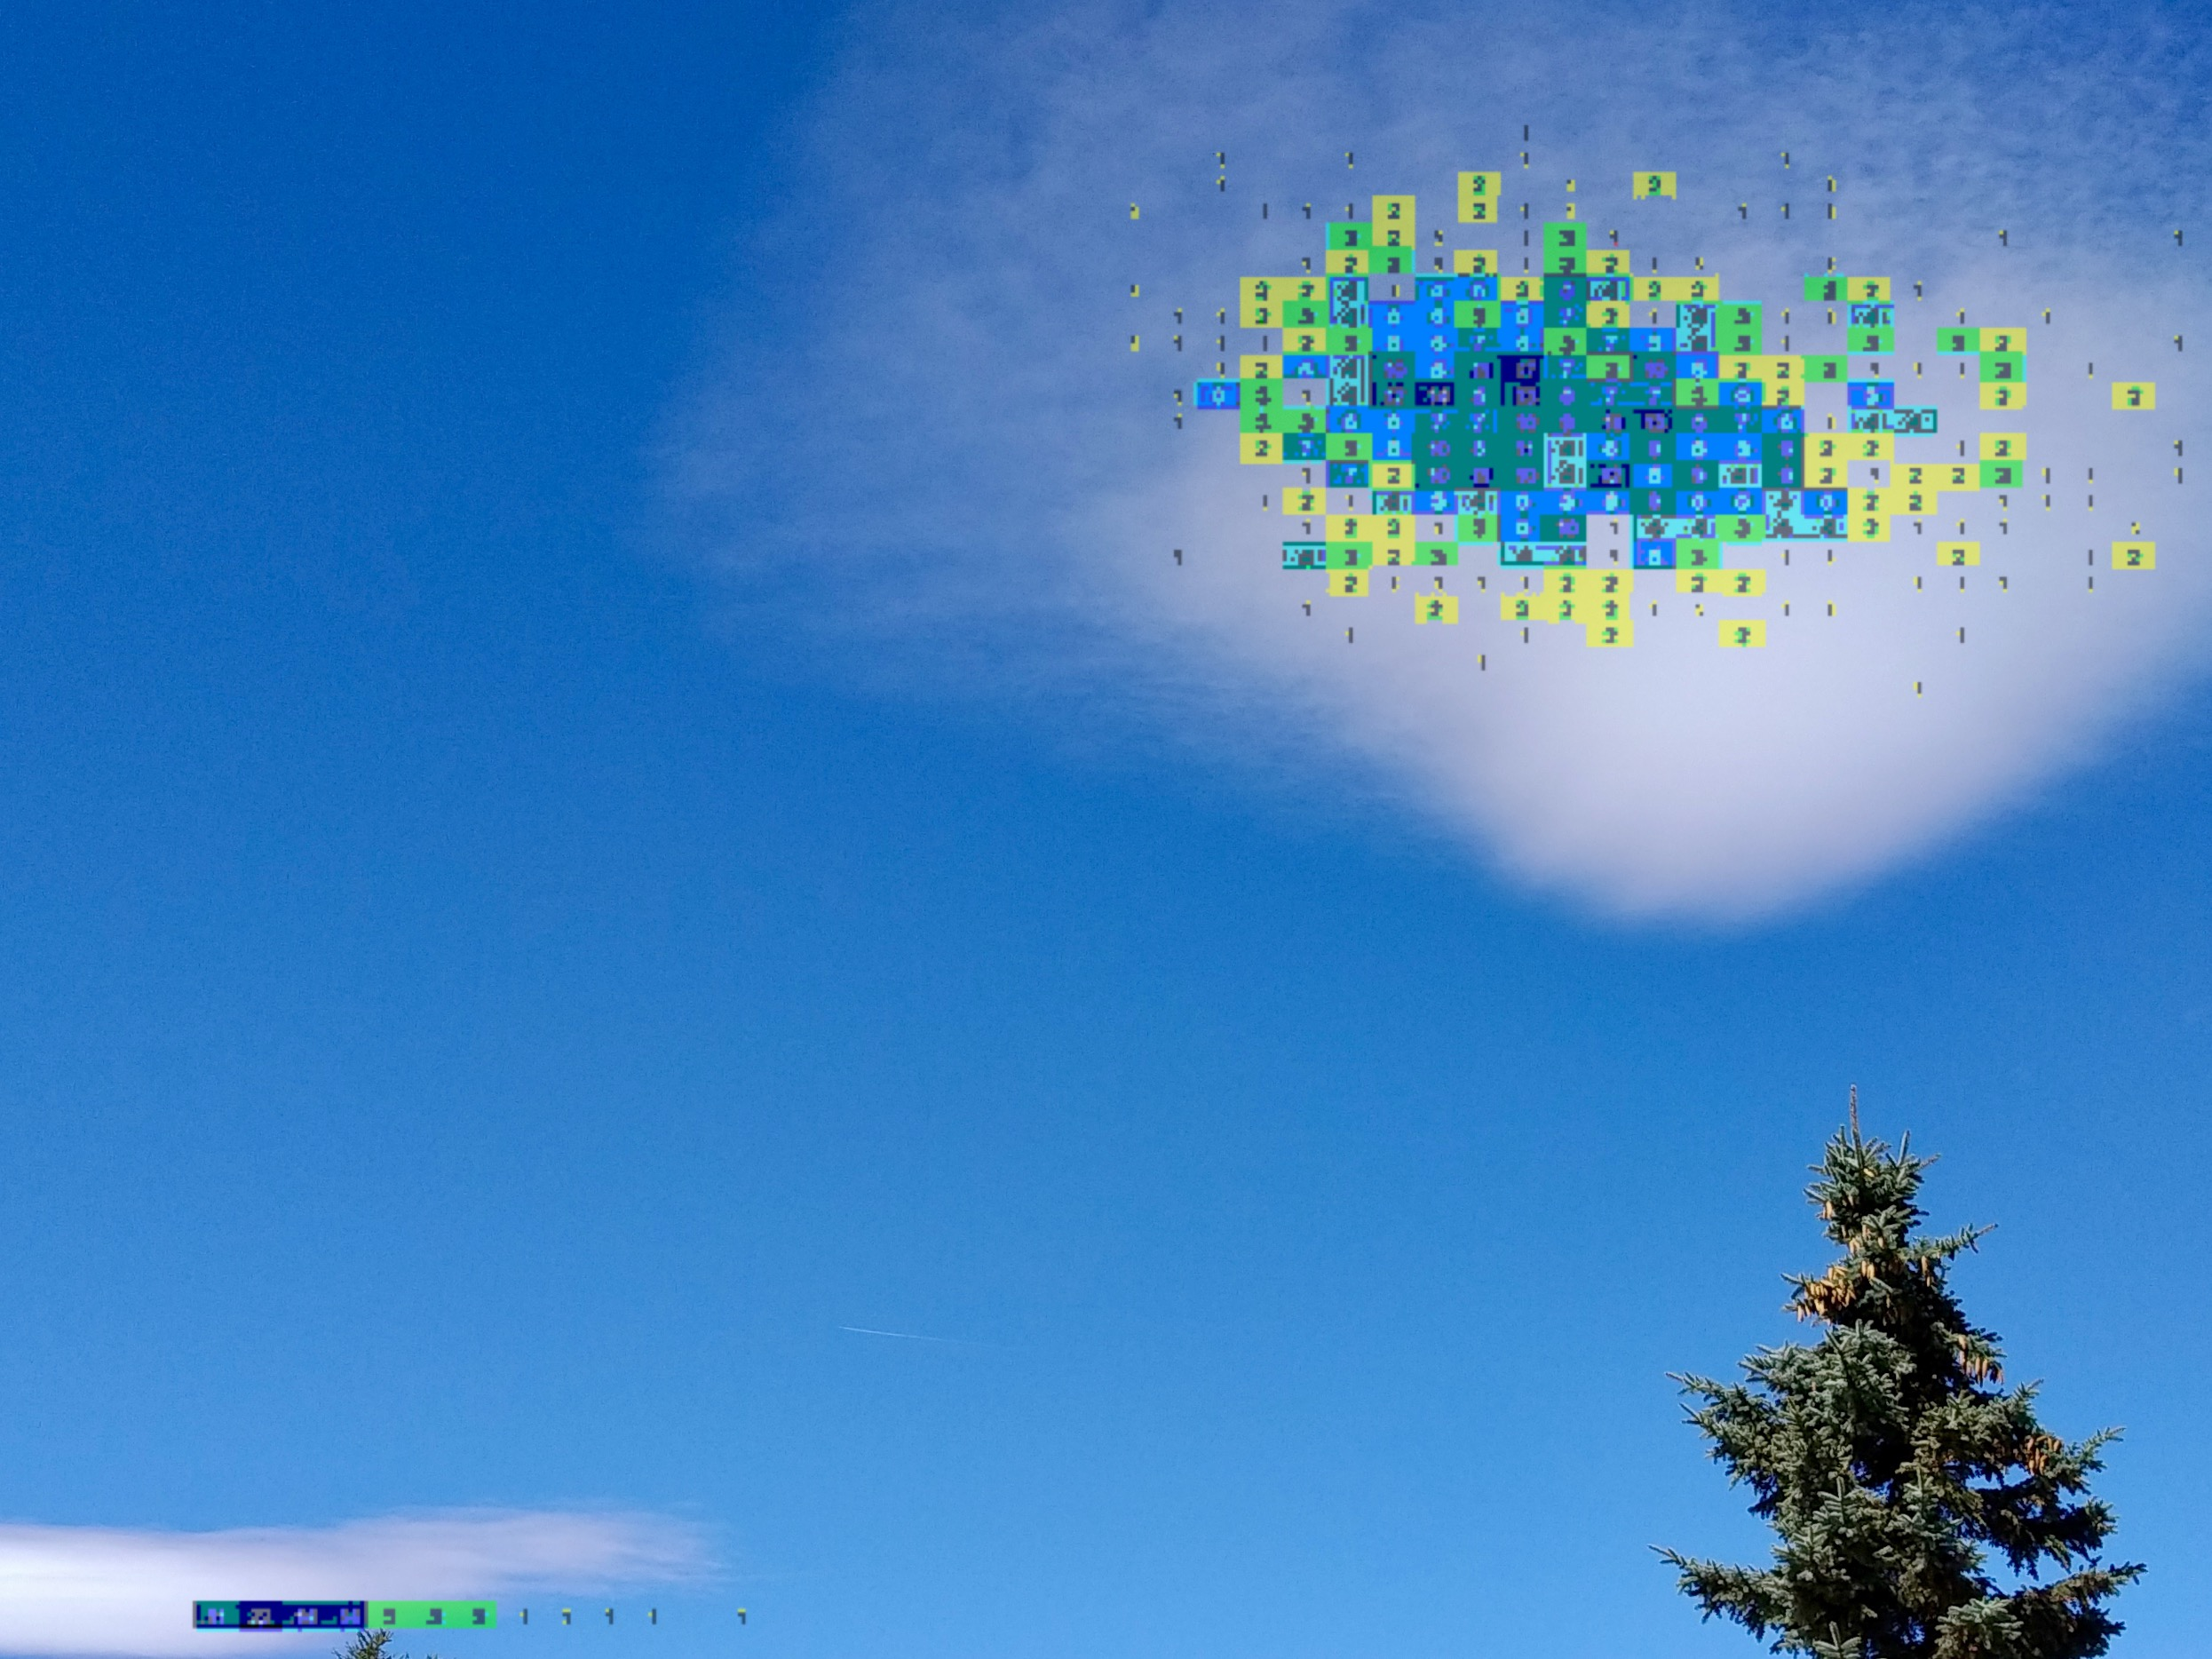
\includegraphics[scale=0.09]{mappaEpidemieNelleNuvole.jpeg}
\end{figure}

\

The image, elaborating Fig. \ref{noCTab}, is dedicated to Pietro Greco (Barano d'Ischia, April $20^{\text{\tiny th}}$, 1955---Ischia, December $18^{\text{\tiny th}}$, 2020)
 
\end{frame}

\end{document}